\documentclass[dvipsnames,table,twoside,11pt]{article}

\usepackage{jsat}
\usepackage{amsmath, amsthm, amssymb}
\usepackage{booktabs}
%\usepackage[pdf]{pstricks}
%\usepackage{pst-tree}
\usepackage{xspace}

%\usepackage[numbers,sort&compress]{natbib}

%\usepackage{showframe}   % debug

\usepackage{pifont}
\usepackage{multirow}
\usepackage{tikz}
\usepackage{subcaption}

\usepackage{listings}
\lstdefinelanguage{smtlib2}
  {alsoletter={-, =},
   morekeywords={set-logic,declare-fun,assert,check-sat,set-info,exit},
   sensitive=false,
   morecomment=[l]{;}}
\lstset{language=smtlib2,
basicstyle=\sffamily,
numbers=none,
keywordstyle=\bfseries\sffamily,
keywordstyle={[2]\bfseries\sffamily\underbar}
}

\newcommand{\rem}[1]{\textcolor{red}{[#1]}}
\newcommand{\todo}[1]{\rem{TODO #1}}

%\input epsf
\special{papersize=8.5in,11in}

\jsatheading{?}{2019}{??-??}
\ShortHeadings{The SMT Competition 2015--2018}
{Weber et al.}
\firstpageno{1}

% macros for tracks for more constistency
\newcommand{\maintrack}{Main Track\xspace}
\newcommand{\apptrack}{Application Track\xspace}
\newcommand{\ucoretrack}{Unsat-Core Track\xspace}

% float layout
\setcounter{topnumber}{2}
\setcounter{bottomnumber}{2}
\setcounter{totalnumber}{4}
\renewcommand{\topfraction}{0.85}
\renewcommand{\bottomfraction}{0.85}
\renewcommand{\textfraction}{0.15}
\renewcommand{\floatpagefraction}{0.7}

\colorlet{bool}{blue!10}
\colorlet{cvc4}{cyan!10}
\colorlet{smti}{yellow!10}
\colorlet{yices}{green!10}
\colorlet{vamp}{orange!10}
\colorlet{q3b}{red!10}
\colorlet{prob}{gray!10}
\colorlet{z}{Fuchsia!10}
\colorlet{coli}{Brown!10}
\colorlet{spass}{Lavender!10}
\colorlet{apr}{PineGreen!10}
\colorlet{rat}{Goldenrod!10}
\colorlet{cvc3}{Melon!10}
\colorlet{redl}{Yellow!10}
\colorlet{alt}{LimeGreen!10}
\colorlet{verit}{MidnightBlue!10}
\colorlet{stp}{Fuchsia!10}
\colorlet{nonc}{black!55}

\newcommand{\cc}[1]{\cellcolor{#1}}
\newcommand{\wc}{\cc{white}}
\newcommand{\rc}[1]{\rowcolor{#1}}
\newcommand{\nc}[1]{{[}#1{]}}

\newcommand{\nonc}{\color{nonc}}

%%%%%%%%%%%%%%%%%%%%%%%%%%%%%%%%%%%%%%%%%%%%%%%%%%%%%%%%%%%%%%%%%%%%%%%%%%%%%%%%

\begin{document}

\title{The SMT Competition 2015--2018}

\author{%
  \name{Tjark Weber {\normalfont (competition chair, 2015--2018)}}
  \email{tjark.weber@it.uu.se} \\
  \addr Uppsala University \\
  %Uppsala \\
  Sweden
  \AND
  \name{Sylvain Conchon {\normalfont (co-organizer, 2015--2016)}}
  \email{Sylvain.Conchon@lri.fr} \\
  \addr Paris-Sud University \\
  France
  \AND
  \name{David D\'{e}harbe {\normalfont (co-organizer, 2015--2016)}}
  \email{david.deharbe@clearsy.com} \\
  \addr ClearSy Systems Engineering \\
  %Aix-en-Provence \\
  France
  \AND
  \name{Matthias Heizmann {\normalfont (co-organizer, 2016--2018)}}
  \email{heizmann@informatik.uni-freiburg.de} \\
  \addr University of Freiburg \\
  %City \\
  Germany
  \AND
  \name{Aina Niemetz {\normalfont (co-organizer, 2018)}}
  \email{niemetz@cs.stanford.edu} \\
  \addr Stanford University\\
  %Stanford \\
  USA
  \AND
  \name{Giles Reger {\normalfont (co-organizer, 2017--2018)}}
  \email{giles.reger@manchester.ac.uk} \\
  \addr University of Manchester \\
  UK}

\maketitle

%%%%%%%%%%%%%%%%%%%%%%%%%%%%%%%%%%%%%%%%%%%%%%%%%%%%%%%%%%%%%%%%%%%%%%%%%%%%%%%%

\begin{abstract}
  The International Satisfiability Modulo Theories Competition is an
  annual competition between Satisfiability Modulo Theories~(SMT)
  solvers.  The 2018 edition of the competition was part of the FLoC
  Olympic Games, which comprised 14 competitions in various areas of
  computational logic.  We report on the design and selected results
  of the SMT Competition during the last FLoC Olympiad, from 2015 to
  2018.  These competitions set several new records regarding the
  number of participants, number of benchmarks used, and amount of
  computation performed.
\end{abstract}

\keywords{SMT solver, SMT-COMP, SMT-LIB, Satisfiability Modulo Theories, competitions}

\published{November 2018}{March 2019}{TBA}

%% Expected content according to the JSAT Call for Papers:

%% Full articles by competition organizers reporting on SAT 2018
%% competitions and evaluation. The articles should describe the
%% competition, its criteria, why it is interesting to the SAT
%% research community, execution environment used, analysis of the
%% results (including how they compare to previous instantiations, if
%% appropriate), and give a summary of the main technical
%% contributions to the field, as well as discussions on lessons
%% learned and suggestions for improvements for future competitions.

%%%%%%%%%%%%%%%%%%%%%%%%%%%%%%%%%%%%%%%%%%%%%%%%%%%%%%%%%%%%%%%%%%%%%%%%%%%%%%%%

%% Changes 2015:
%% \begin{itemize}
%% \item All solvers will be run with $n=4$ cores available.  We will
%%   recognize both best sequential and best parallel performance in all
%%   \maintrack divisions, using different CPU time limits.
%% \item The division scoring will take time spent on unsolved benchmarks
%%   into account.  Previous competitions only considered time spent on
%%   solved benchmarks.  However, the number of solved benchmarks still
%%   takes precedence over run-time.
%% \item In addition to recognizing the best solver in each division, we
%%   will recognize solvers that perform best according to
%%   competition-wide criteria, emphasizing breadth of supported logics.
%%   These criteria will be a refinement of the criteria used for the
%%   FLoC Olympic Games medals in~2014.
%% \item We plan to include new divisions for floating-point arithmetic.
%%   These should be considered experimental in~2015, and will not be
%%   included in the competition-wide ranking.
%% \item We plan to run solvers on all eligible benchmarks.  Previous
%%   competitions used a proper subset of eligible benchmarks, causing
%%   competition results to be affected by a random selection process.
%% \end{itemize}

%% Changes 2016:
%% \begin{itemize}
%% \item Benchmarks will use (a subset of) version~2.5 of the SMT-LIB
%%   language.  \emph{Rationale:} This is the latest version of the
%%   SMT-LIB language.  It was released on 2015-06-28, and is largely
%%   backwards-compatible to version~2.0, which was used for SMT-COMP
%%   2015.
%% \item Solver output may affect the score even when the solver does not
%%   terminate within the time limit.  (In 2015, \maintrack solver output
%%   was ignored if the solver subsequently timed out.)  Solvers should
%%   take care not to accidentally produce output that contains
%%   \texttt{sat} or \texttt{unsat} even when they are killed.
%%   \emph{Rationale:} Users are likely to trust solver responses even
%%   when the solver continues to run for some time.
%% \item Divisions for floating-point arithmetic are no longer
%%   experimental, and will be considered competitive if the necessary
%%   requirements (see Section~\ref{sec:scoring}) are met.
%%   \emph{Rationale:} Floating-point divisions were experimental in
%%   2015.  By now, their definition is sufficiently stable, and they are
%%   supported by several solvers.
%% \item Division scores will be based on a weighted sum of scores for
%%   benchmark families.  \emph{Rationale:} For some years now, SMT-COMPs
%%   have had sufficient computational resources to evaluate all solver
%%   entrants on all eligible benchmarks.  As a side-effect, the
%%   weighting of benchmark families that was achieved in early SMT-COMPs
%%   through a careful selection of benchmarks (based on benchmark
%%   difficulty and category) was lost.  Since there are vast differences
%%   in size between benchmark families, we believe that a weighting that
%%   de-emphasizes large benchmark families (see
%%   Section~\ref{sec:division-scoring}) will lead to more meaningful
%%   competition results.
%% \item The \ucoretrack that was introduced in SMT-COMP 2012, but
%%   discontinued in 2013-2015 (partly because of the competition's move
%%   to StarExec), is back.  It will be experimental in 2016; its results
%%   will be reported, but no official winners will be announced.
%%   \emph{Rationale:} Unsat cores are important in many applications of
%%   SMT solving.  The track was discontinued primarily for
%%   infrastructure and resource reasons.  We are pleased that we can
%%   finally offer it again, but we ask for your understanding in case of
%%   mishaps while we port the required tools.
%% \item Best industrial performance will no longer be recognized
%%   separately.  \emph{Rationale:} While there is agreement in the SMT
%%   community to emphasize problems that come from real applications,
%%   industrial performance largely coincided with overall performance in
%%   SMT-COMP 2015.  We consider the effort to determine and report it
%%   separately no longer justified.
%% \end{itemize}

%% Changes 2017:
%% \begin{itemize}
%% \item Submission of accompanying information for solvers is via a web
%%   form (rather than by email to the organizers).  \emph{Rationale:}
%%   Email submissions were often incomplete, leading to ambiguity and
%%   further inquiries.  The form provides a more structured way of
%%   submitting information.
%% \item Benchmarks will use (a subset of) version~2.6 of the SMT-LIB
%%   language.  \emph{Rationale:} This is the latest version of the
%%   SMT-LIB language.  It is largely backwards-compatible with earlier
%%   versions (in particular~2.0 and~2.5).
%% \item Benchmarks that use partial bit-vector functions, such as
%%   \texttt{bvudiv}, or underspecified floating-point functions, such as
%%   \texttt{fp.min}, will be eligible for the competition again.
%%   \emph{Rationale:} A conclusion on the semantics of these functions
%%   has finally been reached, and the status of affected SMT-LIB
%%   benchmarks has been updated accordingly.
%% \item Benchmarks with unknown status will be eligible for the
%%   competition's \maintrack.  In 2016, solver performance on benchmarks
%%   with unknown status was evaluated but reported separately; in 2017,
%%   it will directly affect the competition results.  \emph{Rationale:}
%%   Using only benchmarks with known status (i.e., benchmarks that have
%%   been solved before) to determine the competition results unjustly
%%   favors imitation of existing solvers over true innovation.
%% \item In the competition-wide scoring, the (per-division) penalty for
%%   erroneous results is changed from the number of errors to a fixed
%%   constant (multiplied by the weight of the respective division).
%%   \emph{Rationale:} The weight already takes the number of benchmarks
%%   in the division into account; multiplying it by the number of errors
%%   overemphasizes large divisions.
%% \item The \ucoretrack, which was re-introduced in 2016, is no
%%   longer experimental.  Its divisions will be considered competitive
%%   if the necessary requirements (see Section~\ref{sec:scoring}) are
%%   met.  \emph{Rationale:} Rules and tool support for the unsat-core
%%   track proved sufficiently stable in 2016.
%% \item The competition will feature experimental divisions for
%%   benchmarks that use algebraic datatypes.  \emph{Rationale:}
%%   Algebraic datatypes are specified in the draft SMT-LIB~2.6 standard,
%%   which is expected to become official in the near future, and are
%%   already supported by some solvers.  Benchmarks that use datatypes
%%   have recently been added to SMT-LIB.
%% \end{itemize}

%% Changes 2018:
%% \begin{itemize}
%% \item The time limit per solver/benchmark pair is anticipated to be at
%%   most 20 minutes in the \maintrack, and at most 40 minutes in the
%%   other tracks.  \emph{Rationale:} Already in 2017, the time limit for
%%   the \maintrack was reduced to 20 minutes (down from 40 minutes in
%%   earlier years) to cope with the inclusion of a large number of
%%   benchmarks with unknown status.
%% \item In the \ucoretrack, the unsatisfiability check for the
%%   returned core will be based on a simple majority vote.  The case
%%   that a solver finds its own core satisfiable will no longer be
%%   treated specially.  \emph{Rationale:} This allows to simplify the
%%   post-processing of \ucoretrack results considerably.
%% \item In 2017, the competition featured experimental divisions for
%%   benchmarks that use algebraic datatypes.  These divisions will be
%%   regular (non-experimental) in 2018. \emph{Rationale:} Algebraic
%%   datatypes are specified in the latest official release (Version~2.6)
%%   of the SMT-LIB standard.
%% \item The competition will feature an experimental divisions for
%%   benchmarks that use strings.  \emph{Rationale:} Corresponding
%%   theories and benchmarks are expected to be added to SMT-LIB in the
%%   near future.
%% \end{itemize}

%%%%%%%%%%%%%%%%%%%%%%%%%%%%%%%%%%%%%%%%%%%%%%%%%%%%%%%%%%%%%%%%%%%%%%%%%%%%%%%%

\section{Introduction}
\label{sec:introduction}

Satisfiability Modulo Theories (SMT) is a generalization of Boolean
satisfiability (SAT), the satisfiability decision problem for
propositional logic.  In place of Boolean variables, SMT formulas may
contain terms that are built from function and predicate symbols drawn
from a number of background theories.  Background theories, which are
motivated by application domains, include the theory of arrays,
integer and real arithmetic, bit-vectors, and floating-point numbers,
among others~\cite{BarFT-RR-17}.  For instance, the following is an
SMT formula over the combination of integer arithmetic and
uninterpreted functions:
%
$$x \leq y \wedge y \leq x \wedge P (f(x) - f(y)) \wedge \neg P(0).$$
%
This formula asserts that~$x$ is less than or equal to~$y$, that~$y$
is less than or equal to~$x$, that~$P$ holds for the difference
of~$f(x)$ and~$f(y)$, and that~$P$ does not hold for~$0$.  (Here,~$x$
and~$y$ are integers,~$f$ is a function from integers to integers,
and~$P$ is a predicate over integers.)
%
Software tools to determine the satisfiability of such formulas are
called SMT solvers.  With its rich input language, SMT has
applications in software engineering, optimization, and many other
areas~\cite{DeMoura:2011:SMT}.

Internally, many SMT solvers employ SAT solving techniques to deal
with the propositional structure of the formula, and combine these
with (semi-)decision procedures for the background theories that the
solver
supports~\cite{DBLP:conf/cav/BarrettCDHJKRT11,DBLP:conf/cade/BoutonODF09,DBLP:conf/tacas/MouraB08,Nieuwenhuis:2006:SSS:1217856.1217859}.
Historically, SMT solvers have focused on quantifier-free formulas and
decidable combinations of background theories.  Increasingly, however,
SMT solvers also support quantified formulas.  Hence there is overlap
between SMT solving and automated theorem proving for quantified
Boolean formulas (QBF), first-order logic, and even higher-order
logic~\cite{DBLP:journals/corr/abs-1712-01486}.

The International Satisfiability Modulo Theories Competition
(SMT-COMP)~\cite{BdMS05,BdMS07,BDdMOS13,BDOS08,BDOS10,CDW14,CGBD12} is
an annual competition between SMT solvers.  It was instituted in~2005,
and is affiliated with the International Workshop on Satisfiability
Modulo Theories.  Solvers are submitted to the competition by their
developers, and pitted against each other in a number of tracks and
divisions.  The SMT Competition was part of the Federated Logic
Conference (FLoC) Olympic Games, which comprised 14 competitions in
various areas of computational logic, in Vienna in~2014, and again in
Oxford~(UK) in~2018.  It was last described in a 2014 competition
report~\cite{CDW14}.  In this paper, we report on the design and
selected results of the competition during the last FLoC Olympiad,
from 2015 to~2018.

Complete data about past competitions since 2015 (and partly for
earlier competitions) is available from the competition website,
\url{http://www.smtcomp.org}.  This includes detailed results for each
solver/benchmark combination, totaling nearly 6 million data records
(about 1.1~GB in CSV format).  Competition solvers and benchmarks may
be downloaded from StarExec, \url{https://www.starexec.org}.

The rest of this paper is structured as follows.  In
Section~\ref{sec:goals}, we present the goals and organization of the
competition.  Section~\ref{sec:smtlib} introduces the SMT-LIB language
and library, and Section~\ref{sec:benchmarks} discusses competition
divisions and benchmarks.  The competition is being run on StarExec,
which is described in Section~\ref{sec:starexec}.
Section~\ref{sec:participants} gives an overview of participating
solvers.  Selected competition results are presented in
Section~\ref{sec:results}, and analyzed in more detail in
Section~\ref{sec:analysis}.  We conclude with suggestions for future
SMT Competitions in Section~\ref{sec:conclusions}.

%%%%%%%%%%%%%%%%%%%%%%%%%%%%%%%%%%%%%%%%%%%%%%%%%%%%%%%%%%%%%%%%%%%%%%%%%%%%%%%%

\section{The Competition Goals and Organization}
\label{sec:goals}

The original goals of the SMT Competition were to spur adoption of the
community-designed SMT-LIB format (see Section~\ref{sec:smtlib}), and
to spark further advances in SMT, especially for
verification~\cite{BdMS05}.  These, together with providing a useful
yardstick of performance for users and developers of SMT solvers, are
still its main goals to date.  The competition has been successful in
establishing SMT-LIB as the de~facto standard language for SMT
solvers.  In recent years, the focus in this regard has shifted
towards promoting some of the newer extensions of the SMT-LIB
language~\cite{BarFT-RR-17}, such as floating-point numbers and
algebraic datatypes.

The competition is organized under the direction of the SMT Steering
Committee, which appoints the competition chair.  (This appointment
should happen ``within 30 days from the end of the current edition of
the SMT workshop''~\cite{smt-bylaws} but in practice has often
happened later.)  The competition chair then assembles a team of
organizers, and oversees the work for the next edition of the
competition.
%
The SMT Workshop includes a block of time to present the competitors
and results of the competition.  The workshop is affiliated with a
major conference in the field of automated reasoning each year: with
CAV in 2015, with IJCAR in 2016, again with CAV in 2017, and with FLoC
in~2018.  Consequently, its date varies.  Competition results were
presented on July~19 in 2015, on July~2 in 2016, on July~23 in 2017,
and on July~13 in~2018.

Important competition deadlines are determined by calculating
backwards from the date of the next SMT Workshop.  The competition's
computational workload should be completed approximately two weeks
before the workshop date.  This gives participants and other parties a
chance to scrutinize the data for errors, allows partial re-runs of
competition jobs if necessary, and gives the organizers time to
prepare the results presentation.  While making all data publicly
available well in advance of the official results presentation may
impact the suspense, it has on several occasions helped to uncover
serious problems with the competition tools or the StarExec framework
(see Section~\ref{sec:starexec}) that could have led to invalid
results otherwise.

It typically takes up to three weeks to run all competition jobs on
the StarExec cluster, so the final submission deadline for solvers
needs to be about five weeks before the workshop date.  The
competition imposes a separate deadline for first versions of solvers
about two weeks before the final submission deadline.  This earlier
deadline has proved useful for the organizers to obtain an accurate
estimate on the number of competing solvers, and to run preliminary
tests with some of the submitted solvers to identify potential issues.
Participants can still make changes to their solver until the final
deadline but are encouraged to use this period for bug-fixing only.

Around the initial solver deadline, the organizers also aim to publish
the latest version of the competition tools, and---in collaboration
with the SMT-LIB maintainers---to release a new version of the SMT
Library (see Section~\ref{sec:smtlib}).  SMT-LIB releases were made on
June~1 in 2015, on May~23 in 2016, on June~5 in 2017, and on May~20 in
2018.  Anyone may submit new benchmarks to the SMT Library, and
competitors are permitted to tune their solvers accordingly.
Therefore all benchmarks eligible for the competition must be released
at least some time before the final solver submission deadline.  To
give the SMT-LIB maintainers sufficient time for curation, the
deadline for new benchmark contributions has usually been about four
to six weeks before the initial solver deadline, typically in April or
early May.

The competition rules are revised each year, and a (near final) draft
version of the rules is made public on the competition website around
mid-April.  The competition chair has ultimate responsibility for the
rules, but changes are often preceded by discussions among the
organizers or within the SMT community.  Such discussions are
initiated by a Call for Comments that is sent out to the SMT-COMP
mailing list~\cite{smtcomp-mailinglist} in February or early March.
Publicly, this call is the first harbinger of a new edition of the SMT
Competition.

%%%%%%%%%%%%%%%%%%%%%%%%%%%%%%%%%%%%%%%%%%%%%%%%%%%%%%%%%%%%%%%%%%%%%%%%%%%%%%%%

\section{The SMT-LIB Language and Library}
\label{sec:smtlib}

All problems used in the SMT Competition come from the SMT Library
(SMT-LIB).  This is a large collection of benchmark problems from
various sources.  The SMT Library is available from a public
repository~\cite{smtlib-repository}, and each new release is mirrored
on StarExec.  Users of SMT solvers are encouraged to submit new and
interesting benchmarks to the library, which has grown from 1,352
benchmarks in~2005~\cite{BdMS05} to 347,011 benchmarks in 2018.

Benchmarks in the SMT Library are written in the SMT-LIB
language~\cite{BarFT-RR-17}, a text-based format that defines the
syntax and semantics of solver input and output.  This includes a
language for terms and formulas, and a command language for
interacting with SMT solvers.  For instance,
Figure~\ref{fig:smtlib-example} shows the example formula from
Section~\ref{sec:introduction} as a benchmark in SMT-LIB syntax, with
commands to the SMT solver typeset in bold.

In~2016, benchmarks were updated from version~2.0 to version~2.5 of
the SMT-LIB language.  Since~2017, benchmarks are written in
version~2.6.  Fortunately, versions~2.5 and~2.6 are largely
backwards-compatible to 2.0, so that older solvers are still able to
compete with at most minor modifications.

\begin{figure}
\begin{lstlisting}
(set-info :smt-lib-version 2.6)
(set-logic QF_UFLIA)
(set-info :status unsat)
(declare-fun x () Int)
(declare-fun y () Int)
(declare-fun f (Int) Int)
(declare-fun P (Int) Bool)
(assert (and (<= x y) (<= y x) (P (- (f x) (f y))) (not (P 0))))
(check-sat)
(exit)
\end{lstlisting}
\caption{A benchmark problem in SMT-LIB syntax.}
\label{fig:smtlib-example}
\end{figure}

The SMT Library classifies benchmarks according to their \emph{logic},
that is, according to the specific combination of background theories
that the benchmark uses.  Logic names are composed of letter groups
that refer to these background theories: {A} or {AX} for the theory of
arrays, {BV} for the theory of bit-vectors, {DT} for algebraic
datatypes, {FP} for the floating-point theory, {IA} for integer
arithmetic, {RA} for real arithmetic, {IRA} for mixed integer and real
arithmetic, {S} for the theory of strings, {UF} for uninterpreted
functions (i.e., free symbols).  Additionally, logics may impose
further syntactic restrictions, such as the absence of quantifiers
({QF\_}), the restriction to difference logic over the
integers~({IDL}) or reals ({RDL}), or to the (non-)linear fragment of
arithmetic ({N} or {L}, respectively, before {IA}, {RA} or {IRA}).
For instance, the logic QF\_UFLIA contains quantifier-free formulas
with uninterpreted functions over linear integer arithmetic.  These
restrictions are typically motivated by the existence of efficient
decision procedures for certain syntactic fragments.

Additionally, the SMT Library distinguishes between \emph{incremental}
and \emph{non-incremental} benchmarks.  Non-incremental benchmarks
contain a single {\tt check-sat} command, which instructs the SMT
solver to determine the satisfiability of the benchmark.  (Valid
solver responses are {\tt sat}, {\tt unsat}, and {\tt unknown}.)
Incremental benchmarks exercise additional solver features, such as
the ability to retract assertions, and typically contain multiple {\tt
  check-sat} commands.  These benchmarks originate from applications
such as bounded model
checking~\cite{Gunther:2014:IBS:2632362.2632374}, where SMT solvers
interact with other tools in a feedback loop.

The 2018 release of the SMT Library contained 336,844 non-incremental
benchmarks in 51 logics, as well as~10,167 incremental benchmarks
(with a total of nearly 32 million {\tt check-sat} commands) in 26
logics.  Table~\ref{table:smtlib} presents further data on the size of
the SMT Library since~2015.  While the library usually grows from one
year to the other because of the inclusion of new benchmarks and
logics, continuous curation efforts may also cause benchmarks to be
removed or reclassified on occasion, thereby causing individual logics
or even the entire library to shrink.  From~2015 to~2018, the total
number of benchmarks has increased by~68\,\%.  The largest benchmark
in the 2018 release had a size of 1,041~MB; the total size of the
release was 91~GB.

\begin{table}
  \caption{Number of benchmarks and logics in the SMT Library}
  \label{table:smtlib}
  \centering
  \begin{tabular}{r@{\ \ }lrrrr}
    \toprule
                               & & \multicolumn{1}{c}{2015} & \multicolumn{1}{c}{2016} & \multicolumn{1}{c}{2017} & \multicolumn{1}{c}{2018} \\
    \midrule
    \multirow{2}{*}{Non-incremental $\{$} & benchmarks & 196375 & 196114 & 258079 & 336844 \\
                                          & logics     &     40 &     40 &     49 &     51 \\
    \multirow{2}{*}{Incremental $\{$}     & benchmarks &  10019 &  10024 &   6262 &  10167 \\
                                          & logics     &     15 &     15 &     22 &     26 \\
    \bottomrule
  \end{tabular}
\end{table}

Benchmarks in the SMT Library are annotated with additional
information, such as the source of the benchmark and its status (i.e.,
whether the benchmark is satisfiable or unsatisfiable) if this is
known.  (For incremental benchmarks, each {\tt check-sat} command has
a separate status annotation.)  To prevent solvers from simply looking
up the benchmark's status in the SMT Library, benchmarks in the
competition are lightly scrambled before they are presented to
solvers~\cite{DBLP:conf/cade/Weber16}.

%%%%%%%%%%%%%%%%%%%%%%%%%%%%%%%%%%%%%%%%%%%%%%%%%%%%%%%%%%%%%%%%%%%%%%%%%%%%%%%%

\section{Competition Divisions and Benchmarks}
\label{sec:benchmarks}

The SMT Competition consists of several tracks.  Each track is further split
into (logic) \emph{divisions}, where each division corresponds to a logic from
the SMT Library.  As indicated in
Tables~\ref{table:smtlib}--\ref{table:divisions}, there are slightly fewer
divisions (Table~\ref{table:divisions}) than logics in the SMT Library
(Table~\ref{table:smtlib}) because not every logic contains benchmarks eligible
for the competition.

\paragraph{Tracks.}
The \emph{\maintrack}, which
has been a staple of the competition since its
inception in 2005, features non-incremental benchmarks.  The
\emph{\apptrack}, which has been part of the competition since
2011~\cite{BDdMOS13}, features incremental benchmarks.  These
benchmarks are passed to each solver one command at a time by a trace
executor, which waits for the solver's response before passing the
next benchmark command (to prevent look-ahead behavior).  The
\emph{\ucoretrack} uses \maintrack benchmarks that are known to
be unsatisfiable, and solvers are evaluated on their ability to find
small unsatisfiable cores (i.e., a small but still unsatisfiable
subset of the benchmark's assertions).  The \ucoretrack had first
been part of the competition in 2012~\cite{CGBD12}, but was then
discontinued partly because of the competition's move to StarExec and
lacking tool support.  It was re-introduced as an experimental track
in 2016, and has been a regular competition track again since~2017.

\paragraph{Divisions.}
Table~\ref{table:divisions} shows the number of divisions in each
track since~2015.  Participants can choose which tracks and divisions
they want to enter, and competition results are reported separately
for each track and division.  Thus, competing solvers do not need to support
all logics, and may or may not support features such as incremental solving
or unsat-core generation.

\paragraph{Eligible Benchmarks.}
Some benchmarks typically have to be
excluded for syntactic reasons: in 2015 and 2016, 11,966 benchmarks
were excluded because they contained partial or underspecified
operations (e.g., bit-vector division) whose precise semantics were
being debated at the time.  Additionally in~2016, one benchmark was
excluded because it contained incorrect status information.  In~2017,
1,104 benchmarks were excluded because their logic had been classified
incorrectly, and 8~benchmarks were excluded because of incorrect or
missing status information.  Moreover, divisions containing datatypes
({DT})---which were new in~2017---were excluded from the Unsat-Core
track because of lacking tool support.  In~2018, 3,603~benchmarks were
excluded because they contained named terms (a feature of the SMT-LIB
language that is not permitted in competition benchmarks), and
5~benchmarks were excluded because of missing status information.

\begin{table}
  \caption{Number of divisions in each competition track}
  \label{table:divisions}
  \centering
  \begin{tabular}{lcccc}
    \toprule
    & 2015 & 2016 & 2017 & 2018 \\
    \midrule
    \maintrack   &  40 & 40 & 49 & 50 \\
    \apptrack    &  14 & 14 & 16 & 21 \\
    \ucoretrack  &  -- & 40 & 41 & 44 \\
    \bottomrule
  \end{tabular}
\end{table}

\paragraph{Benchmark Selection.}
SMT Competitions until~2014 employed a pseudo-random selection process
to further cull the number of benchmarks used in the competition.
However, a 2013 evaluation of SMT-COMP and SMT-LIB found that this
``significantly lessens the ability of a competition to determine
`best' solvers''~\cite{CSW15}. Together with the increased
computational resources available to the competition since its move to
StarExec, this finding prompted a paradigm shift.  Since 2015, the
competition is evaluating all solvers on all eligible benchmarks.
This change had an unintended side effect: the pseudo-random selection
process had been purposely constrained to choose benchmarks from
different benchmark families (that is, groups of benchmarks with
similar characteristics).

\paragraph{Benchmarks with Unknown Status.}
Another paradigm shift concerns the treatment of benchmarks with
unknown status.  Because of the difficulty to judge solver responses
for such benchmarks, SMT Competitions until 2015 only used benchmarks
whose status was known (i.e., that had been solved previously by
existing SMT solvers).  In 2015, 30,717 non-incremental benchmarks
from the SMT Library were not used for the competition because their
status was unknown.  However, this approach was criticized for
imitating existing solvers rather than truly innovating.  In~2016,
the SMT Library contained 29,724 non-incremental benchmarks with
unknown status; solver performance on these was evaluated but reported
separately.  Since 2017, all non-incremental benchmarks are eligible
for the competition's \maintrack regardless of status, and they
directly affect the competition results.  Solver responses for such
benchmarks are assumed to be correct, unless there is a disagreement
between two or more (otherwise sound e.g. on problems with known status) solvers.  Benchmarks with
disagreements are removed from the competition results.  This conservative approach was chosen over a voting system as this situation is expected to be rare as the SMT-LIB organisers go to a significant effort prior to each competition to update the statuses of problems. A manual investigation is therefore preferred over an automated resolution. Disagreements are reported to the solvers involved and in all cases have led to bugs in solvers being identified and fixed. 
In 2016,
there were disagreements on 79 benchmarks; in 2017, only one benchmark
was removed; and in 2018, there were no disagreements between
otherwise sound solvers.

For incremental benchmarks, the situation is different: an incremental
benchmark is ineligible for the \apptrack if its first {\tt
  check-sat} command has unknown status.  Otherwise, the prefix of the
benchmark that only contains {\tt check-sat} commands with known
status is eligible.  The main reason for this difference is that the
competition tools for the \apptrack (in particular, the trace
executor) have not been adapted yet to support {\tt check-sat}
commands with unknown status. Even though the trace executor has now been modified, we cannot check what impact this may have had on previous results without rerunning all tracks as the trace executor drives the solver.

Tables~\ref{table:benchmarks-main-track}--\ref{table:benchmarks-unsat-core-track}
show the number of benchmarks that were used in each competition track
and division since~2015.  A dash indicates that no eligible benchmarks
were available, and hence the corresponding SMT-LIB logic was not
actually a competition division in that track and year.  The size of
divisions varies widely, from just one benchmark in ABVFP to~72,705
benchmarks in QF\_SLIA.

\subsection{Scoring}

Since there are vast differences in size
between benchmark families in the SMT Library, the competition
since~2016 uses a scoring method that assigns a weight to each
\maintrack benchmark in order to de-emphasize large benchmark
families~\cite{rules18}.  A benchmark's weight is computed as $(1 +
\ln F)/F$, where~$F\geq 1$ is the size of the benchmark's family.  The
log scaling seems a reasonable compromise between linearly combining
numbers of benchmarks, which would overemphasize large families, and
simply averaging the fraction of benchmarks solved, which would
overemphasize small families.

\begin{table}
  \caption{Number of benchmarks used in the \maintrack (by division)}
  \label{table:benchmarks-main-track}
  \centering
  \scalebox{.9}[.8]{\begin{tabular}{lrrrr}
    \toprule
    Division & \multicolumn{1}{c}{2015} & \multicolumn{1}{c}{2016} & \multicolumn{1}{c}{2017} & \multicolumn{1}{c}{2018} \\
    \midrule
    ABVFP      &     -- &     -- &      1 &     1 \\
    ALIA       &     42 &     42 &     42 &    42 \\
    AUFBVDTLIA &     -- &     -- &   1709 &  1709 \\
    AUFDTLIA   &     -- &     -- &    728 &   728 \\
    AUFLIA     &      4 &      4 &      4 &     4 \\
    AUFLIRA    &  19849 &  19849 &  20011 & 20011 \\
    AUFNIRA    &   1050 &   1050 &   1480 &  1480 \\
    BV         &     85 &     85 &   5151 &  5751 \\
    BVFP       &     -- &     -- &     24 &    24 \\
    FP         &     -- &     -- &     61 &    61 \\
    LIA        &    201 &    201 &    388 &   388 \\
    LRA        &    339 &    339 &   2419 &  2419 \\
    NIA        &      9 &      9 &     14 &    14 \\
    NRA        &   3788 &   3788 &   3811 &  3813 \\
    QF\_ABV    &  14720 &  14720 &  15061 & 15066 \\
    QF\_ABVFP  &     -- &     -- &  18129 & 18129 \\
    QF\_ALIA   &    134 &    139 &    139 &   139 \\
    QF\_ANIA   &      6 &      8 &      8 &     8 \\
    QF\_AUFBV  &     37 &     37 &     31 &    31 \\
    QF\_AUFLIA &   1009 &   1009 &   1009 &  1009 \\
    QF\_AUFNIA &     21 &     21 &     17 &    17 \\
    QF\_AX     &    551 &    551 &    551 &   551 \\
    QF\_BV     &  26414 &  26414 &  40043 & 40102 \\
    QF\_BVFP   &      7 &      7 &  17215 & 17215 \\
    QF\_DT     &     -- &     -- &   8000 &  8000 \\
    QF\_FP     &  34413 &  34413 &  40302 & 40300 \\
    QF\_IDL    &   2094 &   2094 &   2193 &  2193 \\
    QF\_LIA    &   5839 &   5839 &   6141 &  6947 \\
    QF\_LIRA   &      6 &      6 &      7 &     7 \\
    QF\_LRA    &   1626 &   1626 &   1649 &  1649 \\
    QF\_NIA    &   8475 &   8593 &  23876 & 23876 \\
    QF\_NIRA   &      2 &      2 &      3 &     3 \\
    QF\_NRA    &  10184 &  10245 &  11354 & 11489 \\
    QF\_RDL    &    220 &    220 &    255 &   255 \\
    QF\_SLIA   &     -- &     -- &     -- & 72705 \\
    QF\_UF     &   6649 &   6649 &   6650 &  7423 \\
    QF\_UFBV   &     31 &     31 &     31 &  1224 \\
    QF\_UFIDL  &    441 &    441 &    428 &   428 \\
    QF\_UFLIA  &    598 &    598 &    583 &   583 \\
    QF\_UFLRA  &   1627 &   1627 &   1284 &  1284 \\
    QF\_UFNIA  &      7 &      7 &      7 &     7 \\
    QF\_UFNRA  &     34 &     34 &     36 &    36 \\
    UF         &   2839 &   2839 &   7562 &  7562 \\
    UFBV       &     71 &     71 &    200 &   200 \\
    UFDT       &     -- &     -- &   4535 &  4527 \\
    UFDTLIA    &     -- &     -- &    303 &   303 \\
    UFIDL      &     68 &     68 &     68 &    68 \\
    UFLIA      &   8404 &   8404 &  10137 & 10137 \\
    UFLRA      &     25 &     25 &     15 &    15 \\
    UFNIA      &   2319 &   2319 &   3308 &  3308 \\
    \midrule
    Total      & 154238 & 154424 & 256973 & 333241 \\
    \bottomrule
  \end{tabular}}
\end{table}

\begin{table}
  \caption{Number of benchmarks used in the \apptrack (by division)}
  \label{table:benchmarks-application-track}
  \centering
  \begin{tabular}{lrrrr}
    \toprule
    Division & \multicolumn{1}{c}{2015} & \multicolumn{1}{c}{2016} & \multicolumn{1}{c}{2017} & \multicolumn{1}{c}{2018} \\
    \midrule
    ALIA       &   24 &   24 &   24 &   24 \\
    ANIA       &    3 &    3 &    3 &    3 \\
    AUFNIRA    &   -- &   -- &   -- &  117 \\
    BV         &   -- &   -- &   -- &   17 \\
    LIA        &    6 &    6 &    6 &    6 \\
    QF\_ABV    &   -- &   -- &   -- &   15 \\
    QF\_ALIA   &   44 &   44 &   44 &   44 \\
    QF\_ANIA   &    5 &    5 &    5 &    5 \\
    QF\_AUFBV  &   -- &   -- &   -- &   10 \\
    QF\_AUFLIA &   72 &   72 &   72 &   72 \\
    QF\_BV     &   18 &   18 &   18 &  815 \\
    QF\_BVFP   &   -- &   -- &    2 &    2 \\
    QF\_FP     &   -- &   -- &    2 &    2 \\
    QF\_LIA    &   65 &   69 &   68 &   69 \\
    QF\_LRA    &   10 &   10 &   10 &   10 \\
    QF\_NIA    &   10 &   10 &   10 &   10 \\
    QF\_UFBV   &   -- &   -- &   -- & 2327 \\
    QF\_UFLIA  &  905 &  905 &  780 &  780 \\
    QF\_UFLRA  & 3331 & 3331 & 3056 & 3058 \\
    QF\_UFNIA  &    1 &    1 &    1 &    1 \\
    UFLRA      & 5358 & 5358 & 1870 & 1870 \\
    \midrule
    Total      & 9852 & 9856 & 5971 & 9257 \\
    \bottomrule
  \end{tabular}
\end{table}

\begin{table}
  \caption{Number of benchmarks used in the \ucoretrack (by
    division)}
  \label{table:benchmarks-unsat-core-track}
  \centering
  \scalebox{1}[.91]{\begin{tabular}{lrrr}
    \toprule
    Division & \multicolumn{1}{c}{2016} & \multicolumn{1}{c}{2017} & \multicolumn{1}{c}{2018} \\
    \midrule
    ALIA       &     41 &     41 &     41 \\
    AUFBVDTLIA &     -- &     -- &     25 \\
    AUFLIA     &      3 &      3 &      3 \\
    AUFLIRA    &  19749 &  19771 &  19771 \\
    AUFNIRA    &   1046 &   1050 &   1053 \\
    BV         &     56 &     94 &   4937 \\
    LIA        &    191 &    233 &    233 \\
    LRA        &    319 &   1106 &   1539 \\
    NIA        &      3 &      4 &      4 \\
    NRA        &   3788 &   3801 &   3801 \\
    QF\_ABV    &   4644 &   4673 &   4677 \\
    QF\_ABVFP  &     -- &   3934 &   3934 \\
    QF\_ALIA   &     80 &     80 &     80 \\
    QF\_ANIA   &      8 &      8 &      8 \\
    QF\_AUFBV  &     31 &     25 &     25 \\
    QF\_AUFLIA &    516 &    516 &    516 \\
    QF\_AUFNIA &     15 &     12 &     12 \\
    QF\_AX     &    279 &    279 &    279 \\
    QF\_BV     &  17172 &  23732 &  25700 \\
    QF\_BVFP   &      6 &   3174 &   3174 \\
    QF\_DT     &     -- &     -- &   4422 \\
    QF\_FP     &  17213 &  20028 &  20026 \\
    QF\_IDL    &    816 &    816 &    816 \\
    QF\_LIA    &   2840 &   2844 &   3019 \\
    QF\_LIRA   &      5 &      5 &      5 \\
    QF\_LRA    &    633 &    671 &    683 \\
    QF\_NIA    &    316 &   3130 &   4842 \\
    QF\_NIRA   &      2 &      2 &      2 \\
    QF\_NRA    &   4948 &   5296 &   5357 \\
    QF\_RDL    &    113 &    113 &    113 \\
    QF\_UF     &   4100 &   4101 &   4330 \\
    QF\_UFBV   &     31 &     31 &    575 \\
    QF\_UFIDL  &    335 &    322 &    322 \\
    QF\_UFLIA  &    195 &    183 &    183 \\
    QF\_UFLRA  &    853 &    511 &    511 \\
    QF\_UFNIA  &      7 &      7 &      7 \\
    QF\_UFNRA  &     18 &     11 &     11 \\
    UF         &   2039 &   3316 &   3442 \\
    UFBV       &     53 &     97 &     97 \\
    UFDT       &     -- &     -- &   1863 \\
    UFIDL      &     62 &     57 &     57 \\
    UFLIA      &   8377 &   7714 &   7743 \\
    UFLRA      &     20 &     10 &     10 \\
    UFNIA      &   2318 &   2432 &   2457 \\
    \midrule
    Total      &  93241 & 114233 & 130705 \\
    \bottomrule
  \end{tabular}}
\end{table}

%%%%%%%%%%%%%%%%%%%%%%%%%%%%%%%%%%%%%%%%%%%%%%%%%%%%%%%%%%%%%%%%%%%%%%%%%%%%%%%%

\section{Infrastructure}
\label{sec:starexec}

Since 2014 (and previously for the evaluation in 2013~\cite{CSW15}),
the computational workload of the competition is being run on
StarExec, a ``cross-community infrastructure for logic
solving''~\cite{DBLP:conf/cade/StumpST14} developed at the University
of Iowa and supported by the National Science Foundation.  Each
machine in the StarExec cluster is equipped with two E5-2609 Intel
Xeon processors (10~MiB Cache, 2.4~GHz).  This hardware configuration
has been unchanged since~2013.  Up to two solvers are run
simultaneously on each machine: one solver on each processor, with
four cores available.  Memory usage is limited to~60~GiB per solver.

On the software side, the cluster is running Red Hat Enterprise Linux
Workstation.  The~2015 competition was running on release~6.3
(Santiago, kernel 2.6.32-431).  This was updated to~7.2 (Maipo, kernel
3.10.0-327) before the~2016 competition, and the kernel was further
updated to~3.10.0-514 before the~2017 competition.  The platform
emphasizes stability over bleeding edge technology.  This has on
occasion caused problems with solver binaries that had been compiled
on other Linux distributions and linked against library versions not
(yet) available on the cluster.  Usually, such problems are easily
solved by building the solver on StarExec instead.  The StarExec
developers have made a virtual machine image available to facilitate
this and similar tasks.

Interaction with StarExec is mostly via its web interface,
\url{https://www.starexec.org}.  The interface allows registered users
to upload and share benchmarks and solvers, to create and manage jobs
that apply selected solvers to a selection of benchmarks, and to view
and download job results.  Other features, such as pre-processing of
benchmarks (e.g., for scrambling) and post-processing of solver
output, are also supported.

Jobs consist of individual \emph{job pairs}.  Each job pair
corresponds to a specific solver/benchmark combination.
Figure~\ref{fig:job-pairs} shows the total number of job pairs for the
SMT Competition from~2015 to~2018.  Over this period, the number has
grown by~72\,\%, from~1,028,615 job pairs in~2015 to~1,776,062 job
pairs in~2018.  (This is the number of unique solver/benchmark
combinations that were part of the competition.  The number of job
pairs that were actually run is even higher: test jobs and job pairs
that had to be re-run, e.g., because of issues with the StarExec
infrastructure, are not included.)  For comparison, the~2014
competition only ran~339,714 job pairs~\cite{CDW14}.

Also shown in Figure~\ref{fig:job-pairs} is the total wall-clock time
(summed over all job pairs) for the competition.  This has more than
doubled, from 3.5~years in~2015 to 7.6~years in~2018.  These are
solver run-times only; time that the cluster spent on pre- and
post-processing of benchmarks and solver output or on other auxiliary
tasks is not included.  The increase in~2016 is largely due to the
inclusion of (non-incremental) benchmarks with unknown status; these
were evaluated with a wall-clock time limit of 10~minutes.  In~2017,
when these benchmarks had become eligible for the \maintrack,
\maintrack job pairs were first run with a time limit of 10~minutes.
When it became apparent to the organizers that there were sufficient
resources to increase this limit, job pairs that had timed out were
re-run with a time limit of 20~minutes.  (In this way, about 2.9 years
of wall-clock time in 2017 were spent on job pairs that were then
re-run.  This time is not included in Figure~\ref{fig:job-pairs}.)
Table~\ref{table:time-limits} shows the wall-clock time limits that
were imposed on job pairs for each track and year.

\begin{table}
  \caption{Wall-clock time limits (in minutes)}
  \label{table:time-limits}
  \centering
  \begin{tabular}{lcccc}
    \toprule
    & 2015 & 2016 & 2017 & 2018 \\
    \midrule
    \maintrack   & 40 & 40 & 20\protect\footnotemark & 20 \\
    \apptrack    & 40 & 40 & 40\phantom{$^{1.}$}      & 40 \\
    \ucoretrack  & -- & 40 & 40\phantom{$^{1.}$}      & 40 \\
    \bottomrule
  \end{tabular}
\end{table}
\footnotetext{These job pairs were first run with a time limit of
  10~minutes.  See the text for details.}

StarExec typically reserves between~80 to~150 machines for the SMT
Competition, allowing its workload to be completed within two to three
weeks.

\begin{figure}
  \centering
  \scalebox{.98}{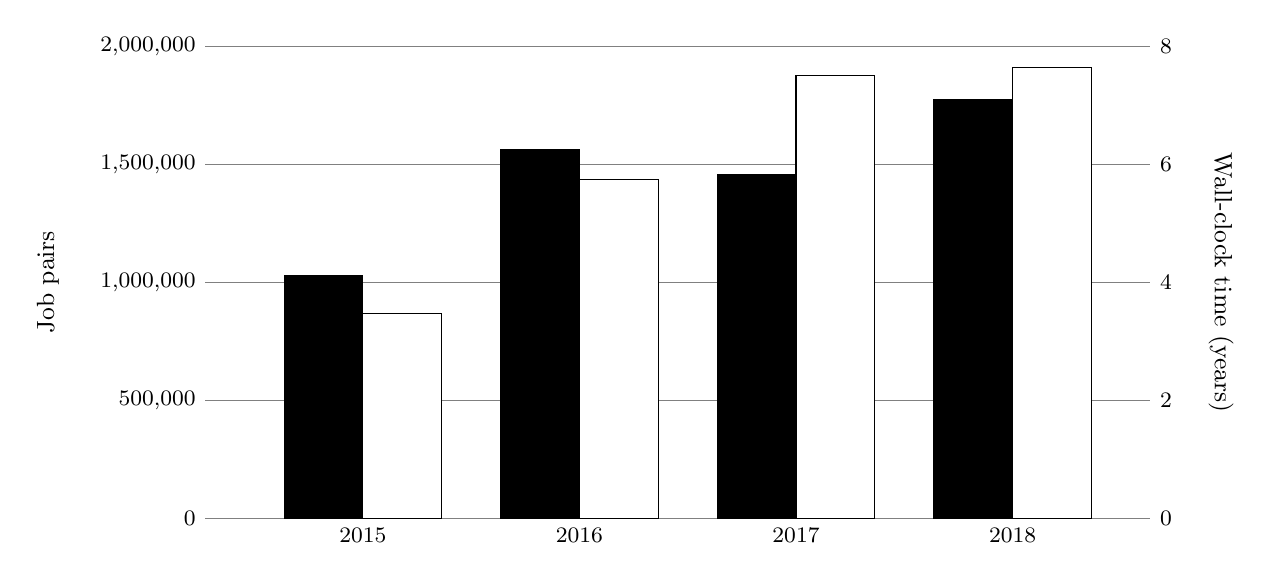
\begin{tikzpicture}
    \draw [gray] (0,0) -- (12,0);
    \draw [gray] (0,1.5) -- (12,1.5);
    \draw [gray] (0,3) -- (12,3);
    \draw [gray] (0,4.5) -- (12,4.5);
    \draw [gray] (0,6) -- (12,6);

    \node [left] at (0,0) {\footnotesize 0};
    \node [left] at (0,1.5) {\footnotesize 500,000};
    \node [left] at (0,3) {\footnotesize 1,000,000};
    \node [left] at (0,4.5) {\footnotesize 1,500,000};
    \node [left] at (0,6) {\footnotesize 2,000,000};

    \node [rotate=90] at (-2,3) {\small Job pairs};

    \node [right] at (12,0) {\footnotesize 0};
    \node [right] at (12,1.5) {\footnotesize 2};
    \node [right] at (12,3) {\footnotesize 4};
    \node [right] at (12,4.5) {\footnotesize 6};
    \node [right] at (12,6) {\footnotesize 8};

    \node [rotate=-90] at (12.9,3) {\small Wall-clock time (years)};

    \draw [fill=black] (1,0) rectangle (2,3.085845); % 1,028,615
    \draw [fill=black] (3.75,0) rectangle (4.75,4.687632); % 1,562,544
    \draw [fill=black] (6.5,0) rectangle (7.5,4.366839); % 1,455,613
    \draw [fill=black] (9.25,0) rectangle (10.25,5.328186); % 1,776,062

    \draw [fill=white] (2,0) rectangle (3,2.6088709094); % 3,4784945459
    \draw [fill=white] (4.75,0) rectangle (5.75,4.3030490392); % 5,7373987189
    \draw [fill=white] (7.5,0) rectangle (8.5,5.6286127759); % 7,5048170345
    \draw [fill=white] (10.25,0) rectangle (11.25,5.7280186691); % 7,6373582255

    \node [below] at (2,0) {\footnotesize 2015};
    \node [below] at (4.75,0) {\footnotesize 2016};
    \node [below] at (7.5,0) {\footnotesize 2017};
    \node [below] at (10.25,0) {\footnotesize 2018};
  \end{tikzpicture}}
  \caption{Number of job pairs ($\blacksquare$) and total wall-clock time ($\square$).}
  \label{fig:job-pairs}
\end{figure}

The use of StarExec ensures the \emph{reproducibility} of the competition. The publicly accessible space \url{https://www.starexec.org/starexec/secure/explore/spaces.jsp?id=2641} stores all of the information required to rerun the competition e.g. all benchmarks and copies of all tools. In addition, a GitHub organisation (\url{https://github.com/SMT-COMP/smt-comp}) has been setup to archive previous results and store the tools used by organisers to run the competition.

%%%%%%%%%%%%%%%%%%%%%%%%%%%%%%%%%%%%%%%%%%%%%%%%%%%%%%%%%%%%%%%%%%%%%%%%%%%%%%%%

\section{Participants}
\label{sec:participants}

Participants must upload their solvers to StarExec to enter them into
the competition, and additionally submit information about each
competing solver---such as the tracks and divisions into which the
solver is being entered---to the competition organizers.  Until 2016,
this information was collected by email.  Since 2017, a web form is
being used for this purpose.  This has greatly reduced the number of
incomplete or ambiguous submissions.

Participants are required to be authors of the tool they submit.
In 2015--2018, the competition rules did not further define authorship,
but it is understood that an author contributed code to the tool.
As a special case of this rule, participants are required to identify
if their tool is a wrapper tool, i.e., any solver that calls (or is in some
other way based on) one or more SMT solvers of which the author of the tool
is not an author.

Tables~\ref{table:participants1}-\ref{table:participants3} list the solvers
that participated between~2015 and~2018, together with contributing team
members (in alphabetical order) and their institutional affiliations (which may
have changed over time).

Further, there was no restriction on the number of solver versions participants
may submit, but the organizers reserved the right to not accept multiple
versions of a solver in case the number of solver submissions is too large for
the computational resources. In the past four years, executing this right was
not necessary.
%
Many of these solvers were submitted in multiple years.  Additionally,
to promote a wide comparison between tools, developers are allowed to
submit multiple versions of a solver, e.g., for different competition
tracks or with differently tuned internal components.
Table~\ref{table:participants-history} shows in more detail how many
versions of each solver were submitted in each year.

Participants were not required to provide source code with their submission.
There were no licensing requirements/restrictions for the submitted binaries
of the participating solvers.
%
Participants were encouraged to submit a short system description
of their solver, including a list of its authors and an explanation of
the SMT solving approach used.  System descriptions are published on
the competition website.  They were submitted for about 60\,\% of all
solver versions since 2015.



{
  \begin{table}
    \centering
    \caption{Participants (2015--2018) Part I} 
    \label{table:participants1}
    \scalebox{.95}{%
    \begin{tabular}{ll}
      \toprule
      Solver & Team Members (Affiliations)\\
      \midrule \midrule
      ABC~\cite{DBLP:conf/cav/BraytonM10}
      & Valeriy Balabanov (Mentor Graphics) \\
      & Robert Brayton (UC Berkeley) \\
      & Alan Mischenko (UC Berkeley)
      \\ \midrule

      Alt-Ergo~\cite{conchon:hal-01960203}
      & Sylvain Conchon (CNRS, University of Paris Sud) \\
      & Albin Coquereau (ENSTA, University of Paris Sud) \\
      & Mohamed Iguernlala (OCamlPro SAS) \\
      & Alain Mebsout (OCamlPro SAS)
      \\ \midrule

      AProVE~\cite{DBLP:journals/jar/GieslABEFFHOPSS17}
      & Cornelius Aschermann (RWTH Aachen University) \\
      & Karsten Behrmann (RWTH Aachen University) \\
      & Marc Brockschmidt (Microsoft Research) \\
      & Andrej Dyck (RWTH Aachen University) \\
      & Fabian Emmes (RWTH Aachen University) \\
      & Florian Frohn (RWTH Aachen University) \\
      & Carsten Fuhs (University College London; Birkbeck, University of London) \\
      & J\"urgen Giesl (RWTH Aachen University) \\
      & Jera Hensel (RWTH Aachen University) \\
      & Patrick Kabasci (RWTH Aachen University) \\
      & Carsten Otto \\
      & Martin Pl\"ucker (RWTH Aachen University) \\
      & Peter Schneider-Kamp (University of Southern Denmark) \\
      & Thomas Str\"oder (RWTH Aachen University) \\
      & Stephanie Swiderski \\
      & Ren\'e Thiemann (University of Innsbruck)
      \\ \midrule

      Boolector~\cite{DBLP:conf/cav/NiemetzPWB18}
      & Armin Biere (Johannes Kepler University) \\
      & Aina Niemetz (Johannes Kepler University, Stanford University) \\
      & Mathias Preiner (Johannes Kepler University, Stanford University)
      \\ \midrule

      COLIBRI~\cite{colibri}
      & Benjamin Blanc (CEA, List) \\
      & Fran\c{c}ois Bobot (CEA, List) \\
      & Zakaria Chihani (CEA, List) \\
      & Bruno Marre (CEA, List) \\
      & Patricia Mouy (CEA, List) \\
      & Franck Vedrine (CEA, List)
      \\ \midrule

      Ctrl-Ergo~\cite{DBLP:conf/cade/BobotCCIMMM12}
      & Mohamed Iguernlala (OCamlPro SAS)
      \\ \midrule

      CVC3~\cite{DBLP:conf/cav/BarrettT07}
      & Kshitij Bansal (New York University) \\
      & Clark Barrett (New York University) \\
      & Morgan Deters (New York University)
      \\ \bottomrule
    \end{tabular}
    }
  \end{table}


  \begin{table}
    \centering
    \caption{Participants (2015--2018) Part II}
    \label{table:participants2}
    \begin{tabular}{ll}
      \toprule
      Solver & Team Members (Affiliations)\\
      \midrule \midrule
      CVC4~\cite{DBLP:conf/cav/BarrettCDHJKRT11}
      & Kshitij Bansal (New Yor University) \\
      & Haniel Barbosa (University of Iowa) \\
      & Clark Barrett (New York University, Stanford University) \\
      & Fran\c{c}ois Bobot (CEA) \\
      & Martin Brain (Oxford University) \\
      & Christopher Conway (Google) \\
      & Morgan Deters (New Yor University) \\
      & Liana Hadarean (Oxford University) \\
      & Duligur Ibeling (Stanford University) \\
      & Dejan Jovanovi\'c (SRI International) \\
      & Timothy King (Verimag) \\
      & Tianyi Liang (University of Iowa) \\
      & Paul Meng (University of Iowa) \\
      & Aina Niemetz (Stanford University) \\
      & Andres N\"otzli (Stanford University) \\
      & Mathias Preiner (Stanford University) \\
      & Andrew Reynolds (EPFL, University of Iowa) \\
      & Cesare Tinelli (University of Iowa)
      \\ \midrule

      MapleSTP
      & Vijay Ganesh (University of Waterloo) \\
      & Jimmy Liang (University of Waterloo)
      \\ \midrule

      MinkeyRink
      & Trevor Hansen (University of Melbourne)
      \\ \midrule

      OpenSMT2~\cite{DBLP:conf/sat/HyvarinenMAS16}
      & Matteo Marescotti (University of Lugano) \\
      & Antti Hyv\"arinen (University of Lugano)
      \\ \midrule

      ProB~\cite{doi:10.1002/9781119002727.ch14}
      & Sebastian Krings (University of D\"usseldorf) \\
      & Michael Leuschel (University of D\"usseldorf)
      \\ \midrule

      Q3B
      & Martin Jon\'a\v{s} (Masaryk University)
      \\ \midrule

      raSAT~\cite{rasat}
      & Mizuhito Ogawa (Japan Advanced Institute of Technology) \\
      & To Van Khanh (Vietnam National University, Hanoi) \\
      & Vu Xuan Tung (Japan Advanced Institute of Technology)
      \\ \midrule

      Redlog~\cite{DBLP:journals/cca/Dolzmann097}
      & Haniel Barbosa (Inria) \\
      & Marek Kosta (Slovak Academy of Sciences, Bratislava)  \\
      & Thomas Sturm (CNRS, MPI Saarbr\"ucken)
      \\ \midrule

      SMT-RAT~\cite{DBLP:conf/sat/CorziliusKJSA15}
      & Erika \'Abrah\'am (RWTH Aachen University) \\
      & Florian Corzilius (RWTH Aachen University) \\
      & Rebecca Haehn (RWTH Aachen University) \\
      & Sebastian Junges (RWTH Aachen University) \\
      & Gereon Kremer (RWTH Aachen University) \\
      & Stefan Schupp (RWTH Aachen University)
      \\ \bottomrule
    \end{tabular}
  \end{table}

  \begin{table}
    \centering
    \caption{Participants (2015--2018) Part III}
    \label{table:participants3}
    \begin{tabular}{ll}
      \toprule
      Solver & Team Members (Affiliations)\\
      \midrule \midrule

      SMTInterpol~\cite{DBLP:conf/spin/ChristHN12}
      & J\"urgen Christ (University of Freiburg) \\
      & Jochen Hoenicke (University of Freiburg) \\
      & Tanja Schindler (University of Freiburg)
      \\ \midrule

      SPASS-SATT~\cite{Bromberger:2019} % TODO update with final bibtex when published
      & Martin Bromberger (Max Planck Institute for Informatics) \\
      & Christoph Weidenbach (Max Planck Institute for Informatics)
      \\ \midrule

      STP~\cite{ganesh07}
      & Vijay Ganesh (University of Waterloo) \\
      & Ryan Govostes (Woods Hole Oceanographic Institute) \\
      & Trevor Hansen (University of Melbourne) \\
      & Dan Liew (Imperial College London) \\
      & Norbert Manthey \\
      & Khoo Yit Phang \\
      & Mate Soos (National University of Singapore)
      \\ \midrule

      toysmt
      & Masahiro Sakai (Toshiba Corporation)
      \\ \midrule

      Vampire~\cite{DBLP:conf/cav/KovacsV13}
      & Evgeny Kotelnikov (Chalmers University) \\
      & Laura Kov\'acs (TU Wien, Chalmers University) \\
      & Giles Reger (University of Manchester) \\
      & Simon Robillard (Chalmers University) \\
      & Martin Suda (University of Manchester, TU Wien) \\
      & Andrei Voronkov (University of Manchester, TU Wien)
      \\ \midrule

      veriT~\cite{DBLP:conf/cade/BoutonODF09}
      & David D\'eharbe (Federal University of Rio Grande do Norte) \\
      & Haniel Barbosa (Inria) \\
      & Pablo Federico Dobal (University of Lorraine) \\
      & Pascal Fontaine (University of Lorraine) \\
      & Daniel El Ouraoui (Inria) \\
      & Hans-J\"org Schurr (Inria)
      \\ \midrule

      %veriT+Redlog~\cite{DBLP:conf/cade/BoutonODF09,DBLP:journals/cca/Dolzmann097}
      %& Haniel Barbosa (Inria) \\
      %& Pascal Fontaine (University of Lorraine) \\
      %& Maximilian Jaroschek (TU Wien) \\
      %& Marek Kosta (Slovak Academy of Sciences, Bratislava)  \\
      %& Thomas Sturm (CNRS, MPI Saarbr\"ucken) \\
      %& Vu Xuan Tung (Japan Advanced Institute of Technology)
      %\\ \midrule

      %veriT+raSAT+Redlog~\cite{DBLP:conf/cade/BoutonODF09,DBLP:journals/cca/Dolzmann097,rasat}
      %& Haniel Barbosa (Inria) \\
      %& Pascal Fontaine (University of Lorraine) \\
      %& Maximilian Jaroschek (TU Wien) \\
      %& Marek Kosta (Slovak Academy of Sciences, Bratislava)  \\
      %& Mizuhito Ogawa (Japan Advanced Institute of Technology) \\
      %& Thomas Sturm (CNRS, MPI Saarbr\"ucken) \\
      %& Vu Xuan Tung (Japan Advanced Institute of Technology)
      %\\ \midrule

      XSat~\cite{DBLP:conf/cav/FuS16}
      & Zhoulai Fu (UC Davis) \\
      & Zhendong Su (UC Davis) \\
      & Martin Velez (UC Davis)
      \\ \midrule

      Yices2~\cite{Dutertre:cav2014}
      & Bruno Dutertre (SRI International) \\
      & Dejan Jovanovi\'c (SRI International) \\
      & Ian Mason (SRI International)
      \\ \midrule

      Z3~\cite{DBLP:conf/tacas/MouraB08}
      & Christoph Wintersteiger (Microsoft Research) \\
      & Aleksandar Zelji\'c (Microsoft Research, Uppsala University)
      \\
      \bottomrule
    \end{tabular}
  \end{table}
}




\begin{table}
  \caption{Number of versions submitted for each solver (by year).
    Numbers in square brackets indicate solver versions that were
    participating hors concours.}
  \label{table:participants-history}
  \centering
  \begin{tabular}{lr@{\,\,}rr@{\,\,}rr@{\,\,}rr@{\,\,}r}
    \toprule
    Solver & \multicolumn{2}{c}{2015} & \multicolumn{2}{c}{2016} & \multicolumn{2}{c}{2017} & \multicolumn{2}{c}{2018} \\
    \midrule
    ABC               &    &      &  2 &      &    &      &    &      \\
    Alt-Ergo          &    &      &    &      &    &      &  1 &      \\
    AProVE            &  1 &      &  1 &      &  1 &      &  1 &      \\
    Boolector         &  3 & [+1] &  2 &      &  2 &      &  2 &      \\
    COLIBRI           &    &      &    &      &  1 &      &  1 &      \\
    Ctrl-Ergo         &    &      &    &      &    &      &  1 &      \\
    CVC3              &  2 &      &    &      &    &      &    &      \\
    CVC4              &  4 &      &  1 & [+1] &  3 &      &  3 & [+1] \\
    MapleSTP          &    &      &  4 &      &    &      &    &      \\
    {[}MathSAT{]}     &    & [+2] &    & [+3] &    & [+3] &    & [+3] \\
    MinkeyRink        &    &      &  1 &      &  1 &      &  2 &      \\
    OpenSMT2          &  2 &      &  1 &      &  1 &      &    & [+1] \\
    ProB              &    &      &  1 &      &    &      &    &      \\
    Q3B               &    &      &  1 &      &  1 &      &  1 &      \\
    raSAT             &  1 &      &  2 &      &    &      &    &      \\
    Redlog            &    &      &    &      &  1 &      &    &      \\
    SMT-RAT           &  2 &      &  1 &      &  1 &      &  2 &      \\
    SMTInterpol       &  1 &      &  1 &      &  1 &      &  1 &      \\
    SPASS-SATT        &    &      &    &      &    &      &  1 &      \\
    STP               &  4 &      &  8 &      &  2 &      &  3 &      \\
    toysmt            &    &      &  1 &      &    &      &    &      \\
    Vampire           &    &      &  2 &      &  1 &      &  1 &      \\
    veriT             &  1 &      &  1 &      &  3 &      &  2 &      \\
    XSat              &    &      &    &      &  1 &      &    &      \\
    Yices2            &  3 &      &  2 &      &  2 &      &  3 &      \\
    Z3                &  2 & [+1] &    & [+1] &    & [+1] &    & [+1] \\
    \midrule
    Total             & 26 & [+4] & 32 & [+5] & 22 & [+4] & 25 & [+6] \\
    \bottomrule
  \end{tabular}
\end{table}

In addition to the solvers that were submitted to the competition by
their respective developers, the organizers included the most recent
stable versions of MathSAT and Z3 for comparison purposes.  Both
solvers are strong tools, but---except for two experimental versions
of Z3 in 2015---their development teams chose not to prepare
competition versions.  These solvers were therefore participating hors
concours.  Moreover, in 2015 a bug was discovered in the \apptrack 
version of Boolector and a fixed version was submitted after the
deadline; in 2016, the CVC4 team did not enter their solver into the
\apptrack; and in 2018, an experimental version of CVC4 as
well as the OpenSMT2 solver were submitted after the deadline.  These
solvers were also participating hors concours.  In result tables, they
are listed with their name in square brackets (e.g., [MathSAT]).

Table~\ref{table:participation-by-track} summarizes these figures and
shows how many solver versions were submitted to each track of the
competition.  Note that solver versions may be entered into multiple
tracks.  Therefore, the total number of solver versions for each year
is typically less than the sum over all tracks.

It can be easy for developers to create multiple versions of their
solver, which may differ only in configuration settings or other minor
details.  We caution against over-interpreting these numbers, which to
some extent depend on how experimental development teams were in any
given year.

By number of solver versions submitted, the competitions in 2015--2018
were the four largest in the history of SMT-COMP.  On average, 26
solver versions were submitted each year since 2015.  In contrast, the
competitions from 2005--2014 only received an average of 12
submissions~\cite{CDW14}.

\begin{table}
  \caption{Participation by track and year.  Numbers in square
    brackets indicate solver versions that were participating hors
    concours.}
  \label{table:participation-by-track}
  \centering
  \begin{tabular}{lr@{\,\,}rr@{\,\,}rr@{\,\,}rr@{\,\,}r}
    \toprule
                      & \multicolumn{2}{c}{2015} & \multicolumn{2}{c}{2016} & \multicolumn{2}{c}{2017} & \multicolumn{2}{c}{2018} \\
    \midrule
    \maintrack   & 21 &               [+2] & 25 & [+2] & 19 & [+2] & 20 & [+4] \\
    \apptrack    & 10 &               [+3] &  8 & [+3] &  4 & [+2] &  4 & [+2] \\
    \ucoretrack  & \multicolumn{2}{c}{---} &  1 & [+4] &  2 & [+2] &  3 & [+2] \\
    \midrule
    Total             & 26 &               [+4] & 32 & [+5] & 22 & [+4] & 25 & [+6] \\
    \bottomrule
  \end{tabular}
\end{table}

%%%%%%%%%%%%%%%%%%%%%%%%%%%%%%%%%%%%%%%%%%%%%%%%%%%%%%%%%%%%%%%%%%%%%%%%%%%%%%%%

\section{Results}
\label{sec:results}

\subsection{Division Rankings}
\label{sec:division-rankings}

Solvers in each division (of each track) are ranked according to a
metric that is based, first, on the number of erroneous responses
(which is usually~0, but solvers that did give erroneous responses are
ranked below solvers that did not); second, on the number of correct
responses; third, on the wall-clock and CPU time that the solver
process consumed.  For the \ucoretrack (which uses unsatisfiable
benchmarks only), the reduction in the size of the unsatisfiable core
is used instead of the number of correct responses.  A detailed
description of the scoring can be found in the competition
rules~\cite{rules18}.

As discussed in Section~\ref{sec:benchmarks}, \maintrack benchmarks
with unknown status are removed from the competition results if two
(or more) solvers that are sound on benchmarks with known status
disagree on their result.  Otherwise, solver responses for benchmarks
with unknown status are assumed to be correct.

All solvers are run with four cores available, and the time limit~$T$
that is imposed on each job pair (see Table~\ref{table:time-limits})
is a wall-clock limit.  Thus, solvers that take advantage of
parallelism might use up to~$4T$ CPU time.  For the \maintrack and the
\ucoretrack, the competition reports parallel and sequential
performance separately.  The latter is determined by imposing a
(virtual) CPU time limit of~$T$.  For the \apptrack, only
parallel performance is reported (because response times to individual
{\tt check-sat} commands are not recorded by StarExec).

A division is \emph{competitive} if
at least two substantially different solvers (i.e., solvers from two
different teams) were submitted.  (Experimental divisions are never
competitive.)  Official winners were declared only for competitive
divisions.

Tables~\ref{tab:winners-main}--\ref{tab:winners-unsat-core} show the
highest-ranked solvers for all (competitive and non-competitive) division from
2015--2018.
We include solvers that were running hors concours (and hence non-competing
and ineligible to be recognized as official competition winners).
Non-com-petitive divisions use gray font.
Entries $A [B]$ indicate that solver $A$ was the highest competing solver,
but non-competing solver $B$ actually ranked best if non-competing solvers
are also taking into consideration.
Entries
$A/B$ indicate that solver~$A$ ranked first considering sequential
performance, while~$B$ ranked first considering parallel performance.
When the same solver ranked first in both, which is most often the
case, its name appears just once.
Table cell colors (other than white) indicate the best competing sequential
solver performance, no cell color indicates that the best sequential solver
performance was by a non-competing solver and no competing solvers participated
in that division.
Full division rankings are available from the competition website.

It is interesting to note that the non-competitive solvers MathSAT and Z3 often appear as the best performing solver. We do not see this as detracting from the overall significance of results. Both solvers are industrial-strength tools, actively maintained and tuned. The reasons for non-entry into the competition are orthogonal to their suitability for the competition. Indeed, Z3 has been entered into the competition competitively in the past and one can assume was trained on the current problems (as much as any solver is). Finally, the fact that industrial-strength solvers perform well in the competition supports the notion that the benchmarks in the competition are industrially relevant.

\begin{table}
\caption{Best \maintrack solvers (by division).}
\label{tab:winners-main}
\centering
\scalebox{.82}{%
\renewcommand{\arraystretch}{1.01}%
  \begin{tabular}{r@{\hskip 1em}>{\columncolor{white}[.25em][.5em]}c@{\hskip 1em}>{\columncolor{white}[.5em][.5em]}c@{\hskip 1em}>{\columncolor{white}[.5em][.5em]}c@{\hskip 1em}>{\columncolor{white}[.5em][0.5em]}c}
    \toprule
    Division         &  2015                        &  2016                     &  2017                           &  2018                     \\
    \hline \hline
    \wc ABVFP        &                              &                           &                                 & \nonc \cc{cvc4} {CVC4}    \\
    \rc{cvc4}
    \wc ALIA         & CVC4 \nc{Z3}                 & CVC4 \nc{Z3}              & CVC4 \nc{Z3}                    & CVC4 \nc{Z3}              \\
    \wc AUFBVDTLIA   &                              &                           & \nonc \cc{cvc4} {CVC4}          & \nonc \cc{cvc4} {CVC4}    \\
    \wc AUFDTLIA     &                              &                           & \nonc \cc{cvc4} {CVC4}          & \cc{cvc4} {CVC4}          \\
    \rc{cvc4}
    \wc AUFLIA       & {CVC4}                       & {CVC4}                    & {CVC4}                          & {CVC4}                    \\
    \rc{vamp}
    \wc AUFLIRA      & \cc{cvc4} CVC4 \nc{Z3}       & Vampire \nc{Z3}           & Vampire \nc{Z3}                 & \cc{cvc4} CVC4 \nc{Z3}    \\
    \rc{vamp}
    \wc AUFNIRA      & \nonc \cc{cvc4} {CVC4}       & {Vampire}                 & {Vampire}                       & \cc{cvc4} {CVC4}          \\
    \rc{q3b}
    \wc BV           & \nonc \cc{cvc4} CVC4 \nc{Z3} & {Q3B}                     & Q3B \nc{Z3}                     & \cc{cvc4} {CVC4}          \\
    \wc BVFP         &                              &                           &                                 & \nonc \cc{cvc4} {CVC4}    \\
    \wc FP           &                              &                           &                                 & \nonc \cc{cvc4} {CVC4}    \\
    \rc{cvc4}
    \wc LIA          & {CVC4}                       & {CVC4}                    & CVC4 \nc{Z3}                    & CVC4 \nc{Z3}              \\
    \rc{cvc4}
    \wc LRA          & {CVC4}                       & {CVC4}                    & CVC4 \nc{Z3}                    & CVC4 \nc{Z3}              \\
    \rc{cvc4}
    \wc NIA          & \nonc CVC4 \nc{Z3}           & \cc{prob} ProB \nc{Z3}    & CVC4 \nc{Z3}                    & CVC4 \nc{Z3}              \\
    \rc{vamp}
    \wc NRA          & \nonc \cc{cvc4} {CVC4}       & {Vampire}                 & \cc{redl} {Redlog}              & Vampire \nc{Z3} / Vampire \\
    \rc{bool}
    \wc QF\_ABV      & {Boolector}                  & {Boolector}               & {Boolector}                     & {Boolector}               \\
    \wc QF\_ABVFP    &                              &                           & {---}                           & \cc{cvc4} {CVC4}          \\
    \rc{yices}
    \wc QF\_ALIA     & {Yices2}                     & {Yices2}                  & {Yices2}                        & {Yices2}                  \\
    \rc{cvc4}
    \wc QF\_ANIA     & \nonc CVC4 \nc{Z3}           & \nonc {CVC4}                & \nonc {CVC4}                  & \nonc CVC4 \nc{Z3}        \\
    \rc{cvc4}
    \wc QF\_AUFBV    & CVC4 \nc{MathSAT}            & CVC4 \nc{MathSAT}         & \cc{yices} Yices2 \nc{MathSAT}  & {CVC4}                    \\
    \rc{yices}
    \wc QF\_AUFLIA   & {Yices2}                     & {Yices2}                  & {Yices2}                        & {Yices2}                  \\
    \rc{cvc4}
    \wc QF\_AUFNIA   & \nonc {CVC4}                 & \nonc {CVC4}              & \nonc CVC4 \nc{Z3}              & \nonc CVC4 \nc{Z3}        \\
    \rc{yices}
    \wc QF\_AX       & {Yices2}                     & {Yices2}                  & {Yices2}                        & {Yices2}                  \\
    \rc{bool}
    \wc QF\_BV       & {Boolector}                  & {Boolector}               & {Boolector/MinkeyRink}          & {Boolector/MinkeyRink}    \\
    \wc QF\_BVFP     & \nonc \cc{z} {Z3}            & \nonc \wc \nc{Z3}         & \nonc \cc{coli} COLIBRI \nc{Z3} & \cc{cvc4} {CVC4}          \\
    \wc QF\_DT       &                              &                           & \nonc \cc{cvc4} {CVC4}          & \nonc \cc{cvc4} {CVC4}    \\
    \rc{coli}
    \wc QF\_FP       & \nonc \cc{z} {Z3}            & \nonc \wc \nc{MathSAT}    & COLIBRI \nc{Z3}                 & {COLIBRI}                 \\
    \rc{yices}
    \wc QF\_IDL      & Yices2 \nc{Z3}               & Yices2 \nc{Z3}            & {Yices2}                        & {Yices2}                  \\
    \rc{cvc4}
    \wc QF\_LIA      & CVC4 \nc{MathSAT}            & CVC4 \nc{MathSAT}         & CVC4 \nc{MathSAT}               & \cc{spass} {SPASS-SATT}   \\
    \rc{yices}
    \wc QF\_LIRA     & {Yices2}                     & {Yices2}                  & Yices2 \nc{Z3}                  & Yices2 \nc{Z3}            \\
    \rc{cvc4}
    \wc QF\_LRA      &  {CVC4}                      & {CVC4}                    & {CVC4}                          & {CVC4}                    \\
    \rc{cvc4}
    \wc QF\_NIA      & \cc{apr} AProVE \nc{Z3}      & \cc{yices} Yices2 \nc{Z3} & {CVC4}                          & {CVC4}                    \\
    \rc{cvc4}
    \wc QF\_NIRA     & {CVC4}                       & {CVC4}                    & \cc{rat} {SMT-RAT}              & \cc{rat} {SMT-RAT}        \\
    \rc{yices}
    \wc QF\_NRA      & Yices2 \nc{Z3}               & Yices2 \nc{Z3}            & {Yices2}                        & Yices2 \nc{Z3}            \\
    \rc{yices}
    \wc QF\_RDL      & {Yices2}                     & {Yices2}                  & {Yices2}                        & {Yices2}                  \\
    \wc QF\_SLIA     &                              &                           &                                 & \nonc \cc{cvc4} {CVC4}    \\
    \rc{yices}
    \wc QF\_UF       & {Yices2}                     & {Yices2}                  & {Yices2}                        & {Yices2}                  \\
    \rc{bool}
    \wc QF\_UFBV     & {Boolector}                  & {Boolector}               & {Boolector}                     & {Boolector}               \\
    \rc{yices}
    \wc QF\_UFIDL    & {Yices2}                     & {Yices2}                  & {Yices2}                        & {Yices2}                  \\
    \rc{yices}
    \wc QF\_UFLIA    & Yices2 \nc{Z3}               & Yices2 \nc{Z3}            & {Yices2}                        & {Yices2}                  \\
    \rc{yices}
    \wc QF\_UFLRA    & {Yices2}                     & {Yices2}                  & {Yices2}                        & {Yices2}                  \\
    \rc{yices}
    \wc QF\_UFNIA    & \nonc \cc{cvc4} {CVC4}       & {Yices2/CVC4}             & {Yices2}                        & {Yices2}                  \\
    \rc{yices}
    \wc QF\_UFNRA    & \nonc \cc{cvc3} CVC3 \nc{Z3} & {Yices2}                  & Yices2 \nc{Z3}                  & {Yices2}                  \\
    \rc{cvc4}
    \wc UF           & {CVC4}                       & {CVC4}                    & \cc{vamp} {Vampire}             &  {CVC4/Vampire}           \\
    \rc{cvc4}
    \wc UFBV         & \nonc CVC4 \nc{Z3}           & CVC4 \nc{Z3}              & \nonc CVC4 \nc{Z3}              & \nonc CVC4 \nc{Z3}        \\
    \wc UFDT         &                              &                           & \nonc \cc{cvc4} {CVC4}          & \cc{cvc4} {CVC4}          \\
    \wc UFDTLIA      &                              &                           & \nonc \cc{vamp} {Vampire}       & \cc{cvc4} {CVC4}          \\
    \rc{cvc4}
    \wc UFIDL        & CVC4 \nc{Z3}                 & {CVC4}                    & {CVC4}                          & CVC4 \nc{Z3}              \\
    \rc{cvc4}
    \wc UFLIA        & {CVC4}                       & {CVC4}                    & {CVC4}                          & {CVC4}                    \\
    \rc{cvc4}
    \wc UFLRA        & \cc{cvc3} {CVC3}             & \cc{vamp} Vampire \nc{Z3} & CVC4 \nc{Z3}                    & CVC4 \nc{Z3}              \\
    \rc{vamp}
    \wc UFNIA        & \nonc \cc{cvc4} {CVC4}       & {Vampire}                 & {Vampire}                       & Vampire \nc{Z3} / Vampire \\
    \bottomrule
  \end{tabular}}
\end{table}


\begin{table}
  \caption{Best \apptrack solvers (by division)}
  \label{tab:winners-application}
  \centering
  \scalebox{.805}{%
  \begin{tabular}{r@{\hskip 1em}>{\columncolor{white}[.25em][.5em]}c@{\hskip 1em}>{\columncolor{white}[.5em][.5em]}c@{\hskip 1em}>{\columncolor{white}[.5em][.5em]}c@{\hskip 1em}>{\columncolor{white}[.5em][0.5em]}c}
    \toprule
    \rc{white}
    Division        & 2015                           & 2016                      & 2017                     & 2018                           \\
    \midrule
    \rc{cvc4}
    \wc ALIA        & \nonc CVC4 \nc{Z3}             & \nonc \wc \nc{Z3}         & \nonc CVC4 \nc{Z3}       & \nonc CVC4 \nc{Z3}             \\
    \rc{cvc4}
    \wc ANIA        & \nonc CVC4 \nc{Z3}             & \nonc \wc \nc{Z3}         & \nonc CVC4               & \nonc CVC4                     \\
    \wc AUFNIRA     &                                &                           &                          & \nonc \cc{cvc4} CVC4           \\
    \wc BV          &                                &                           &                          & \nonc \cc{cvc4} CVC4 \nc{Z3}   \\
    \rc{cvc4}
    \wc LIA         & \nonc CVC4 \nc{Z3}             & \nonc \wc \nc{Z3}         & \nonc CVC4 \nc{Z3}       & \nonc CVC4 \nc{Z3}             \\
    \wc QF\_ABV     &                                &                           &                          & \cc{bool} Boolector            \\
    \rc{smti}
    \wc QF\_ALIA    & \cc{yices} Yices2 \nc{Z3}      & SMTInterpol \nc{Z3}       & SMTInterpol \nc{Z3}      & SMTInterpol \nc{Z3}            \\
    \rc{cvc4}
    \wc QF\_ANIA    & \nonc CVC4 \nc{Z3}             & \nonc \wc \nc{Z3}         & \nonc CVC4 \nc{Z3}       & \nonc CVC4 \nc{Z3}             \\
    \wc QF\_AUFBV   &                                &                           &                          & \cc{yices} Yices2              \\
    \rc{yices}
    \wc QF\_AUFLIA  & Yices2                         & Yices2                    & Yices2                   & Yices2                         \\
    \rc{yices}
    \wc QF\_BV      & Yices2 \nc{MathSAT}            & Yices2 \nc{MathSAT}       & Yices2 \nc{MathSAT}      & Yices2 \nc{MathSAT}            \\
    \wc QF\_BVFP    &                                &                           & \nonc \wc \nc{Z3}        & \nonc \cc{cvc4} CVC4           \\
    \wc QF\_FP      &                                &                           & \nonc \wc \nc{Z3}        & \nonc \cc{cvc4} CVC4 \nc{Z3}   \\

    \rc{yices}
    \wc QF\_LIA     & Yices2                         & Yices2                    & Yices2                   & Yices2                         \\
    \rc{smti}
    \wc QF\_LRA     & \cc{yices} Yices2 \nc{MathSAT} & SMTInterpol \nc{MathSAT}  & SMTInterpol \nc{MathSAT} & \cc{yices} Yices2 \nc{MathSAT} \\
    \rc{cvc4}
    \wc QF\_NIA     & \nonc CVC4 \nc{Z3}             & \nonc \wc \nc{CVC4}       & \nonc CVC4               & CVC4                           \\
    \wc QF\_UFBV    &                                &                           &                          & \cc{bool} Boolector            \\
    \rc{cvc4}
    \wc QF\_UFLIA   & CVC4 \nc{Z3}                   & \cc{yices} Yices2 \nc{Z3} & CVC4 \nc{Z3}             & \cc{smti} SMTInterpol \nc{Z3}  \\
    \rc{yices}
    \wc QF\_UFLRA   & Yices2 \nc{Z3}                 & Yices2 \nc{Z3}            & Yices2                   & Yices2 \nc{Z3}                 \\
    \rc{cvc4}
    \wc QF\_UFNIA   & \nonc CVC4 \nc{Z3}             & \nonc \wc \nc{Z3}         & \nonc CVC4 \nc{Z3}       & CVC4 \nc{Z3}                   \\
    \rc{cvc4}
    \wc UFLRA       & \nonc CVC4 \nc{Z3}             & \nonc \wc \nc{Z3}         & \nonc CVC4 \nc{Z3}       & \nonc CVC4 \nc{Z3}             \\
    \bottomrule
  \end{tabular}
  }
\end{table}


\begin{table}
  \caption{Best unsat-core track solvers (by division)}
  \label{tab:winners-unsat-core}
  \centering
  \scalebox{.93}{\begin{tabular}{rccc}
    \toprule
    Division                        & 2016                               & 2017                                      & 2018                             \\ \midrule \cline{2-4}
    \multicolumn{1}{r|}{ALIA}       & \multicolumn{3}{c|}{{[}Z3{]}}                                                                                     \\ \cline{2-4} 
    AUFBVDTLIA                      &                                    &                                           & \multicolumn{1}{|c|}{CVC4}         \\ \cline{2-4} 
    \multicolumn{1}{r|}{AUFLIA}     & \multicolumn{2}{c|}{{[}Z3{]}}                                                  & \multicolumn{1}{c|}{CVC4}        \\ \cline{2-4} 
    \multicolumn{1}{r|}{AUFLIRA}    & \multicolumn{2}{c|}{{[}Z3{]}}                                                  & \multicolumn{1}{c|}{CVC4}        \\ \cline{2-4} 
    \multicolumn{1}{r|}{AUFNIRA}    & \multicolumn{1}{c|}{{[}Z3{]}}     & \multicolumn{2}{c|}{CVC4}                                                    \\ \cline{2-4} 
    \multicolumn{1}{r|}{BV}         & \multicolumn{3}{c|}{{[}Z3{]}}                                                                                     \\ \cline{2-4} 
    \multicolumn{1}{r|}{LIA}        & \multicolumn{1}{c|}{[veriT]}      & \multicolumn{1}{c|}{CVC4}                 & \multicolumn{1}{c|}{{[}Z3{]}}    \\ \cline{2-4} 
    \multicolumn{1}{r|}{LRA}        & \multicolumn{1}{c|}{[veriT]}      & \multicolumn{2}{c|}{CVC4}                                                     \\ \cline{2-4} 
    \multicolumn{1}{r|}{NIA}        & \multicolumn{1}{c|}{{[}Z3{]}}     & \multicolumn{1}{c|}{CVC4/{[}Z3{]}}        & \multicolumn{1}{c|}{CVC4}        \\ \cline{2-4} 
    \multicolumn{1}{r|}{NRA}        & \multicolumn{3}{c|}{{[}Z3{]}}                                                                                     \\ \cline{2-4} 
    \multicolumn{1}{r|}{QF\_ABV}    & \multicolumn{2}{c|}{{[}Z3{]}}                                                  & \multicolumn{1}{c|}{Yices2}      \\ \cline{2-4} 
    QF\_ABVFP                        &                                   & \multicolumn{1}{|c|}{---}                 & \multicolumn{1}{|c|}{CVC4}        \\ \cline{2-4} 
    \multicolumn{1}{r|}{QF\_ALIA}   & \multicolumn{3}{c|}{{[}Z3{]}}                                                                                     \\ \cline{2-4} 
    \multicolumn{1}{r|}{QF\_ANIA}   & \multicolumn{1}{c|}{{[}Z3{]}}      & \multicolumn{2}{c|}{CVC4}                                                    \\ \cline{2-4} 
    \multicolumn{1}{r|}{QF\_AUFBV}  & \multicolumn{1}{c|}{{[}Z3{]}}      & \multicolumn{2}{c|}{{[}MathSAT{]}}                                           \\ \cline{2-4} 
    \multicolumn{1}{r|}{QF\_AUFLIA} & \multicolumn{1}{c|}{{[}Z3{]}}      & \multicolumn{2}{c|}{CVC4}                                                    \\ \cline{2-4} 
    \multicolumn{1}{r|}{QF\_AUFNIA} & \multicolumn{3}{c|}{{[}Z3{]}}                                                                                     \\ \cline{2-4} 
    \multicolumn{1}{r|}{QF\_AX}     & \multicolumn{2}{c|}{{[}Z3{]}}                                                  & \multicolumn{1}{c|}{Yices2}      \\ \cline{2-4} 
    \multicolumn{1}{r|}{QF\_BV}     & \multicolumn{2}{c|}{{[}MathSAT{]}}                                             & \multicolumn{1}{c|}{Yices2}      \\ \cline{2-4} 
    \multicolumn{1}{r|}{QF\_BVFP}   & \multicolumn{2}{c|}{{[}Z3{]}}                                                  & \multicolumn{1}{c|}{CVC4}        \\ \cline{2-4} 
    QF\_DT                           &                                    &                                           & \multicolumn{1}{|c|}{CVC4}       \\ \cline{2-4} 
    \multicolumn{1}{r|}{QF\_FP}     & \multicolumn{1}{c|}{{[}MathSAT{]}} & \multicolumn{1}{c|}{{[}Z3{]}}             & \multicolumn{1}{c|}{CVC4}        \\ \cline{2-4} 
    \multicolumn{1}{r|}{QF\_IDL}    & \multicolumn{3}{c|}{{[}Z3{]}}                                                                                     \\ \cline{2-4} 
    \multicolumn{1}{r|}{QF\_LIA}    & \multicolumn{1}{c|}{{[}Z3{]}}      & \multicolumn{1}{c|}{SMTInterpol/{[}Z3{]}} & \multicolumn{1}{c|}{SMTInterpol} \\ \cline{2-4} 
    \multicolumn{1}{r|}{QF\_LIRA}   & \multicolumn{3}{c|}{{[}Z3{]}}                                                                                     \\ \cline{2-4} 
    \multicolumn{1}{r|}{QF\_LRA}    & \multicolumn{3}{c|}{SMTInterpol}                                                                                  \\ \cline{2-4} 
    \multicolumn{1}{r|}{QF\_NIA}    & \multicolumn{3}{c|}{{[}Z3{]}}                                                                                     \\ \cline{2-4} 
    \multicolumn{1}{r|}{QF\_NIRA}   & \multicolumn{3}{c|}{{[}Z3{]}}                                                                                     \\ \cline{2-4} 
    \multicolumn{1}{r|}{QF\_NRA}    & \multicolumn{1}{c|}{{[}Z3{]}}      & \multicolumn{2}{c|}{CVC4}                                                    \\ \cline{2-4} 
    \multicolumn{1}{r|}{QF\_RDL}    & \multicolumn{1}{c|}{{[}veriT{]}}   & \multicolumn{2}{c|}{{[}Z3{]}}                                                \\ \cline{2-4} 
    \multicolumn{1}{r|}{QF\_UF}     & \multicolumn{1}{c|}{{[}MathSAT{]}} & \multicolumn{2}{c|}{CVC4}                                                    \\ \cline{2-4} 
    \multicolumn{1}{r|}{QF\_UFBV}   & \multicolumn{2}{c|}{{[}MathSAT{]}}                                             & \multicolumn{1}{c|}{{[}Z3{]}}    \\ \cline{2-4} 
    \multicolumn{1}{r|}{QF\_UFIDL}  & \multicolumn{2}{c|}{{[}Z3{]}}                                                  & \multicolumn{1}{c|}{Yices2}      \\ \cline{2-4} 
    \multicolumn{1}{r|}{QF\_UFLIA}  & \multicolumn{1}{c|}{{[}MathSAT{]}} & \multicolumn{2}{c|}{{[}Z3{]}}                                                \\ \cline{2-4} 
    \multicolumn{1}{r|}{QF\_UFLRA}  & \multicolumn{1}{c|}{{[}Z3{]}}      & \multicolumn{2}{|c|}{{[}MathSAT{]}}                                          \\ \cline{2-4} 
    \multicolumn{1}{r|}{QF\_UFNIA}  & \multicolumn{3}{c|}{{[}Z3{]}}                                                                                     \\ \cline{2-4} 
    \multicolumn{1}{r|}{QF\_UFNRA}  & \multicolumn{3}{c|}{{[}Z3{]}}                                                                                     \\ \cline{2-4} 
    \multicolumn{1}{r|}{UF}         & \multicolumn{1}{c|}{{[}Z3{]}}      & \multicolumn{2}{c|}{CVC4}                                                    \\ \cline{2-4} 
    \multicolumn{1}{r|}{UFBV}       & \multicolumn{2}{c|}{{[}Z3{]}}                                                  & \multicolumn{1}{c|}{CVC4}        \\ \cline{2-4} 
    UFDT                             &                                    &                                           & \multicolumn{1}{|c|}{CVC4}       \\ \cline{2-4} 
    \multicolumn{1}{r|}{UFIDL}      & \multicolumn{1}{c|}{{[}Z3{]}}      & \multicolumn{2}{c|}{CVC4}                                                    \\ \cline{2-4} 
    \multicolumn{1}{r|}{UFLIA}      & \multicolumn{1}{c|}{{[}Z3{]}}      & \multicolumn{2}{c|}{CVC4}                                                    \\ \cline{2-4} 
    \multicolumn{1}{r|}{UFLRA}      & \multicolumn{3}{c|}{{[}Z3{]}}                                                                                     \\ \cline{2-4} 
    \multicolumn{1}{r|}{UFNIA}      & \multicolumn{1}{c|}{{[}Z3{]}}      & \multicolumn{2}{c|}{CVC4}                                                    \\ \cline{2-4} \bottomrule
  \end{tabular}}
\end{table}


%%%%%%%%%%%%%%%%%%%%%%%%%%%%%%%%%%%%%%%%%%%%%%%%%%%%%%%%%%%%%%%%%%%%%%%%%%%%%%%%

\subsection{Competition-Wide Ranking}
\label{sec:floc}

In 2014, the SMT Competition was part of the FLoC Olympic Games, which
sponsored three Kurt G\"odel medals.  These were awarded to the winner
of the \maintrack's QF\_BV division (which had historically been the
logic with the largest number of solver submissions and job pairs), as
well as to the two best \maintrack solvers according to a
competition-wide ranking that had been instituted especially for this
purpose~\cite{CDW14}.  This ranking combines each solver's performance
across all competitive \maintrack divisions into a single score,
giving more weight to larger divisions, and to solvers that solve a
large fraction of the benchmarks~\cite{rules18}.  It emphasizes
breadth of solver participation---a solver participating in many
logics does not need to be the best in any one of them to rank highly.

The competition-wide ranking for the \maintrack was retained and
refined after~2014.  Table~\ref{table:competition-wide-ranking} shows
the best three solvers according to this ranking for 2015--2018.  Also
shown is Z3, which ranked highly each year but was running hors
concours.  Sequential and parallel performance are reported
separately.
%
Note that scores are not directly comparable between different years:
the set of benchmarks changes from one year to the other, and also the
formula to compute the score changed (see below).  Moreover, readers
should keep in mind that this ranking---like any method that maps the
performance of solvers for a broad range of logics to a
one-dimensional value---is inherently limited.  We refer to the
individual division rankings (Section~\ref{sec:division-rankings}) for
more detailed information about each solver.

\begin{table}
  \caption{Competition-wide ranking for the \maintrack: best solvers (by year)}
  \label{table:competition-wide-ranking}
  \centering
  \scalebox{.89}{\begin{tabular}{cp{2.2cm}rrp{0cm}cp{2.2cm}rr}
    \cmidrule[\heavyrulewidth]{1-4} \cmidrule[\heavyrulewidth]{6-9}
    \multicolumn{4}{c}{2015} & & \multicolumn{4}{c}{2016} \\ \cmidrule{1-4} \cmidrule{6-9}
    Rank & Solver & Score  & Score  & & Rank & Solver & Score & Score \\
         &        & (sequential) & (parallel) & & & & (sequential) & (parallel) \\ \cmidrule{1-4} \cmidrule{6-9}
         & [Z3]              & 159.36 & 159.36 & &    & [Z3]   & 185.09 & 185.09 \\
      1. & CVC4              & 144.67 & 144.74 & & 1. & CVC4   & 180.95 & 181.19 \\
      2. & CVC4(exp)\footnotemark & 140.47 & 140.51 & & 2. & Yices2 & 119.29 & 119.29 \\
      3. & Yices             & 101.91 & 101.91 & & 3. & veriT  &  75.11 &  75.11 \\ \cmidrule[\heavyrulewidth]{1-4} \cmidrule[\heavyrulewidth]{6-9}
  \end{tabular}}

  \medskip

  \scalebox{.89}{\begin{tabular}{cp{2.2cm}rrp{0cm}cp{2.2cm}rr}
    \cmidrule[\heavyrulewidth]{1-4} \cmidrule[\heavyrulewidth]{6-9}
    \multicolumn{4}{c}{2017} & & \multicolumn{4}{c}{2018} \\ \cmidrule{1-4} \cmidrule{6-9}
    Rank & Solver & Score  & Score  & & Rank & Solver & Score & Score \\
         &        & (sequential) & (parallel) & & & & (sequential) & (parallel) \\ \cmidrule{1-4} \cmidrule{6-9}
         & [Z3]        & 171.99 & 171.99 & & 1. & CVC4        & 211.99 & 211.99 \\
      1. & CVC4        & 161.38 & 161.76 & &    & [Z3]        & 186.19 & 186.19 \\
      2. & Yices2      & 110.63 & 110.63 & & 2. & Yices2      & 115.26 & 115.26 \\
      3. & SMTInterpol &  65.96 &  66.00 & & 3. & SMTInterpol &  65.32 &  65.38 \\ \cmidrule[\heavyrulewidth]{1-4} \cmidrule[\heavyrulewidth]{6-9}
  \end{tabular}}
\end{table}
\footnotetext{This was a distinct version of CVC4 that was designated as experimental.}

A contentious issue with this ranking has been the scoring of
incorrect solver responses.  In the division rankings, an incorrect
response causes a solver to be ranked below all correct solvers for
that division.  But the competition's \maintrack consists of many
independent divisions.  A solver bug that affects one division need
not manifest itself in other divisions.  To balance the strong
interest in correct solvers against the risk of stifling innovation,
the competition-wide ranking was revised in~2017 to use a fixed
numeric penalty for each division with incorrect responses.  The value
of this penalty is currently set so that entering a (possibly buggy)
solver that can solve all benchmarks into a division has a positive
expected score if the probability that a soundness bug in the solver
will be triggered is below~$20\,\%$.~\cite{rules18}

The 2018 edition of the competition was again part of the FLoC Olympic
Games, which sponsored seven medals.  The competition organizers
awarded the following solvers:
\begin{itemize}
\item The best three \maintrack solvers according to the
  competition-wide ranking (CVC4, Yices2, and SMTInterpol; see
  Table~\ref{table:competition-wide-ranking}),
\item the solvers that won the QF\_BV division in the \maintrack 
  (Boolector and MinkeyRink; see Table~\ref{tab:winners-main}),
\item the solver that won the most competitive divisions in the
  \apptrack (Yices2),
\item the solver that won the most competitive divisions in the
  \ucoretrack (Yices2).
\end{itemize}

In comparison to the competition-wide ranking for the \maintrack, the
metric used for the \apptrack and \ucoretrack---simply counting
the number of competitive divisions that a solver has won---was rather
unsophisticated.  Future editions of the competition should perhaps
refine this to use a ranking scheme that is more similar to the
\maintrack ranking, by weighing divisions according to their relative
importance, and also by rewarding good performance from solvers other
than division winners.  A difficulty in adapting the \maintrack
ranking for the other tracks is that each \maintrack benchmark is
worth one point (before benchmark weights are applied) if solved
correctly, while benchmarks in the \apptrack and \ucoretrack
are worth widely varying numbers of points.  Moreover, in the
\ucoretrack, the size of the smallest unsatisfiable core---and
hence the number of points attainable on any given benchmark---may not
be known precisely.

%%%%%%%%%%%%%%%%%%%%%%%%%%%%%%%%%%%%%%%%%%%%%%%%%%%%%%%%%%%%%%%%%%%%%%%%%%%%%%%%

\begin{figure}
  \centering
  \scalebox{.45}{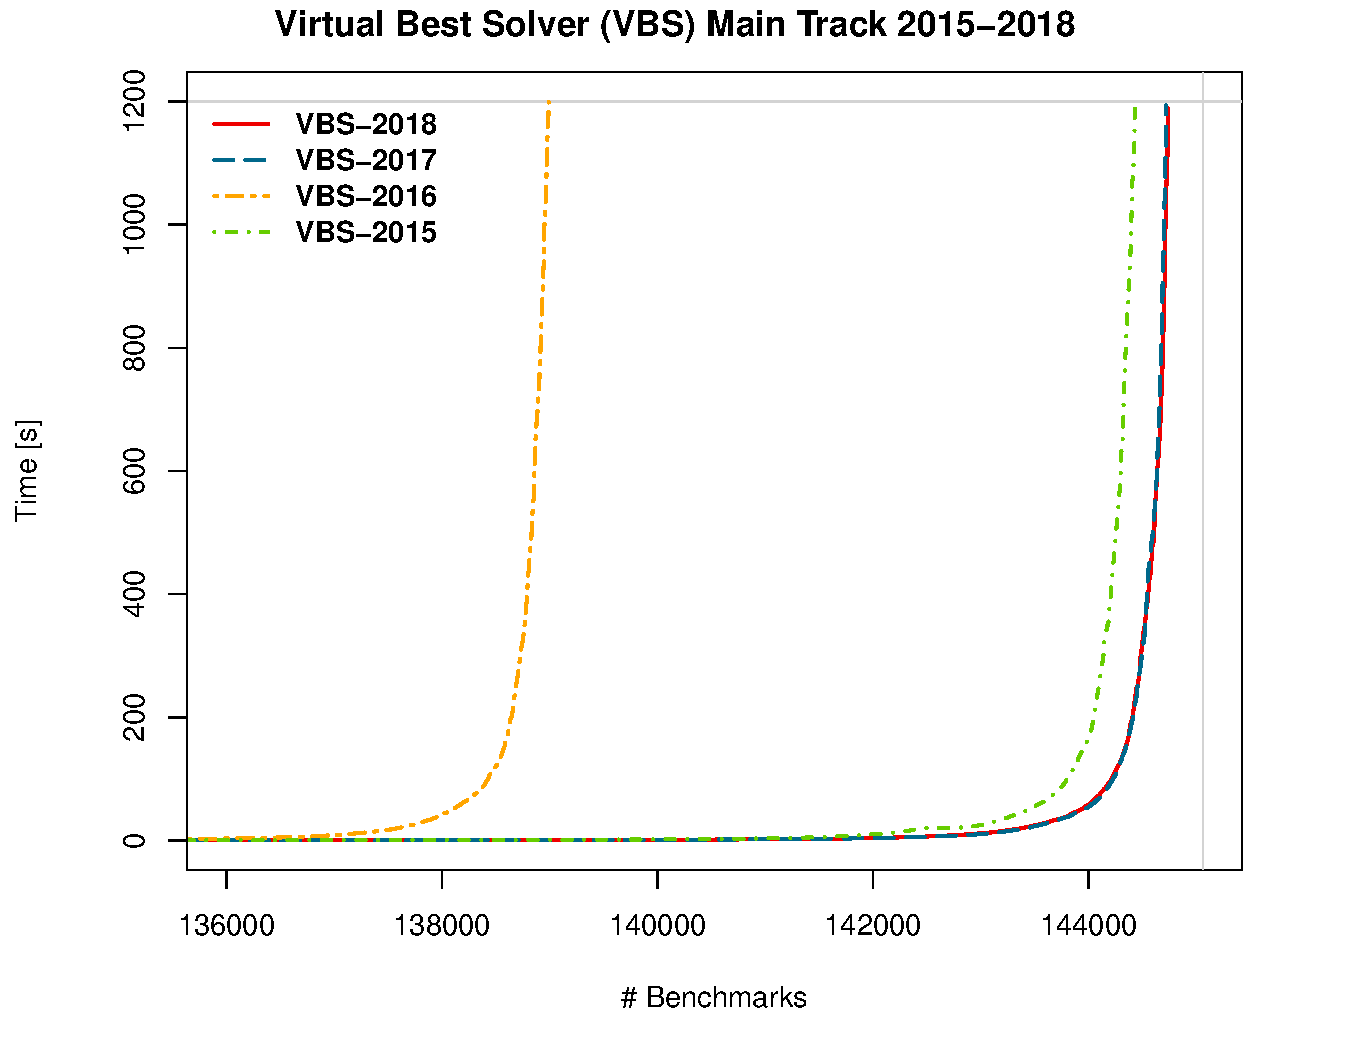
\includegraphics{%
        plot/pdf/cactus_plot-Virtual_Best_Solver_(VBS)_Main_Track_2015-2018.pdf}}
  \caption{VBS on common benchmarks 2015-2018 of all logics in the \maintrack 
  with a time limit of 1200s. Number of common benchmarks is indicated with a
  gray vertical line.}
  \label{fig:progress-all}
\end{figure}

\begin{figure}
  \begin{subfigure}[t]{0.5\textwidth}
    \scalebox{.35}{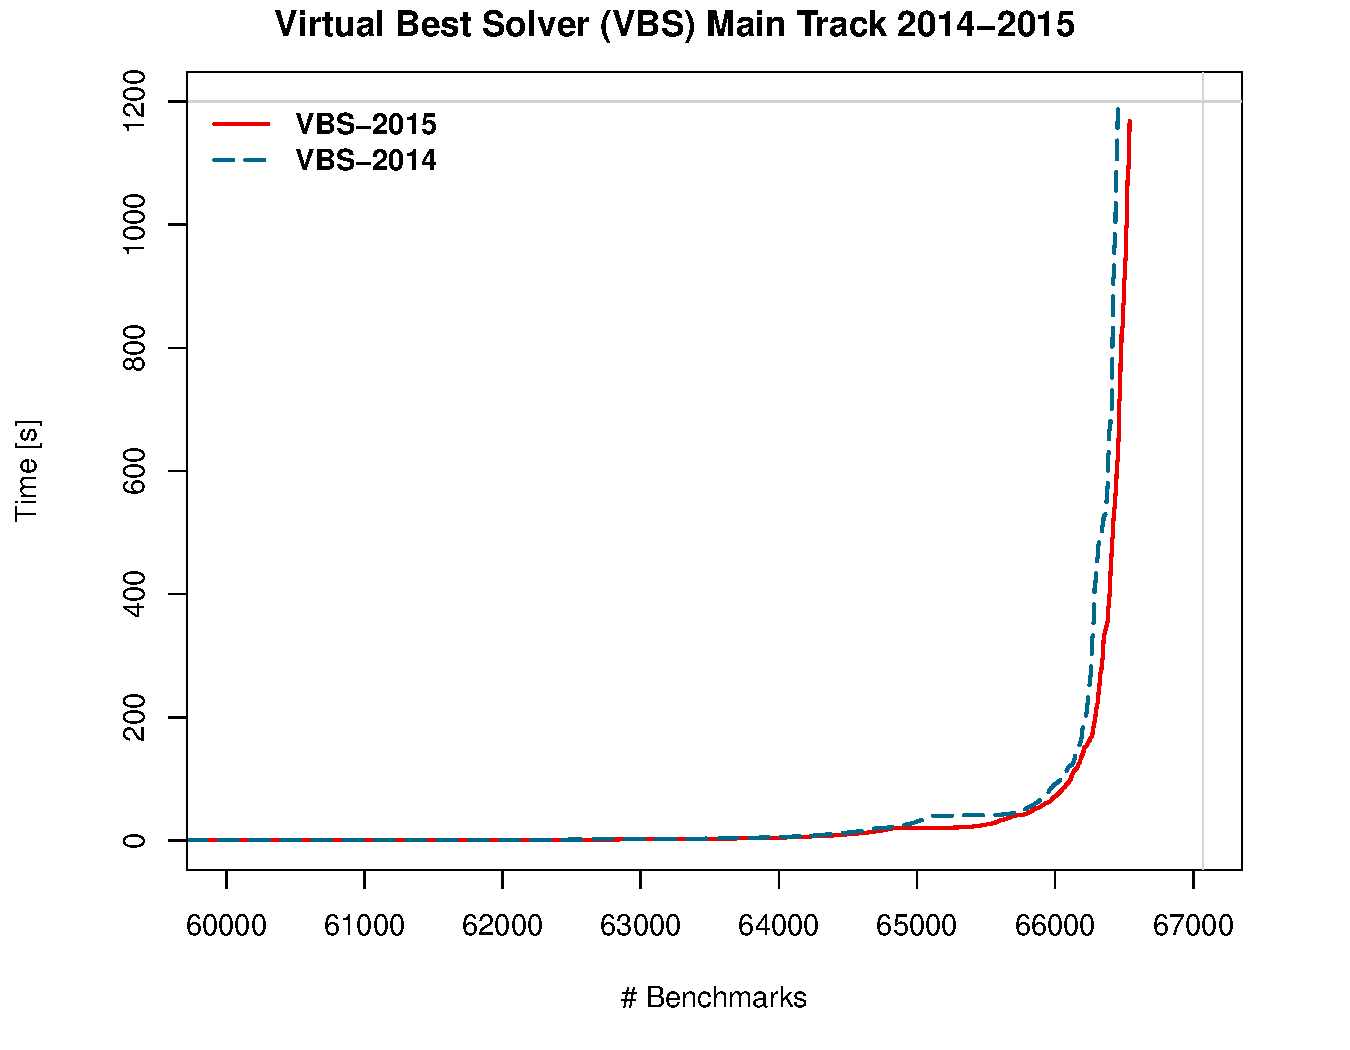
\includegraphics{%
        plot/pdf/cactus_plot-Virtual_Best_Solver_(VBS)_Main_Track_2014-2015.pdf}}
    \caption{2014 vs.~2015}
  \end{subfigure}
  \begin{subfigure}[t]{0.5\textwidth}
    \scalebox{.35}{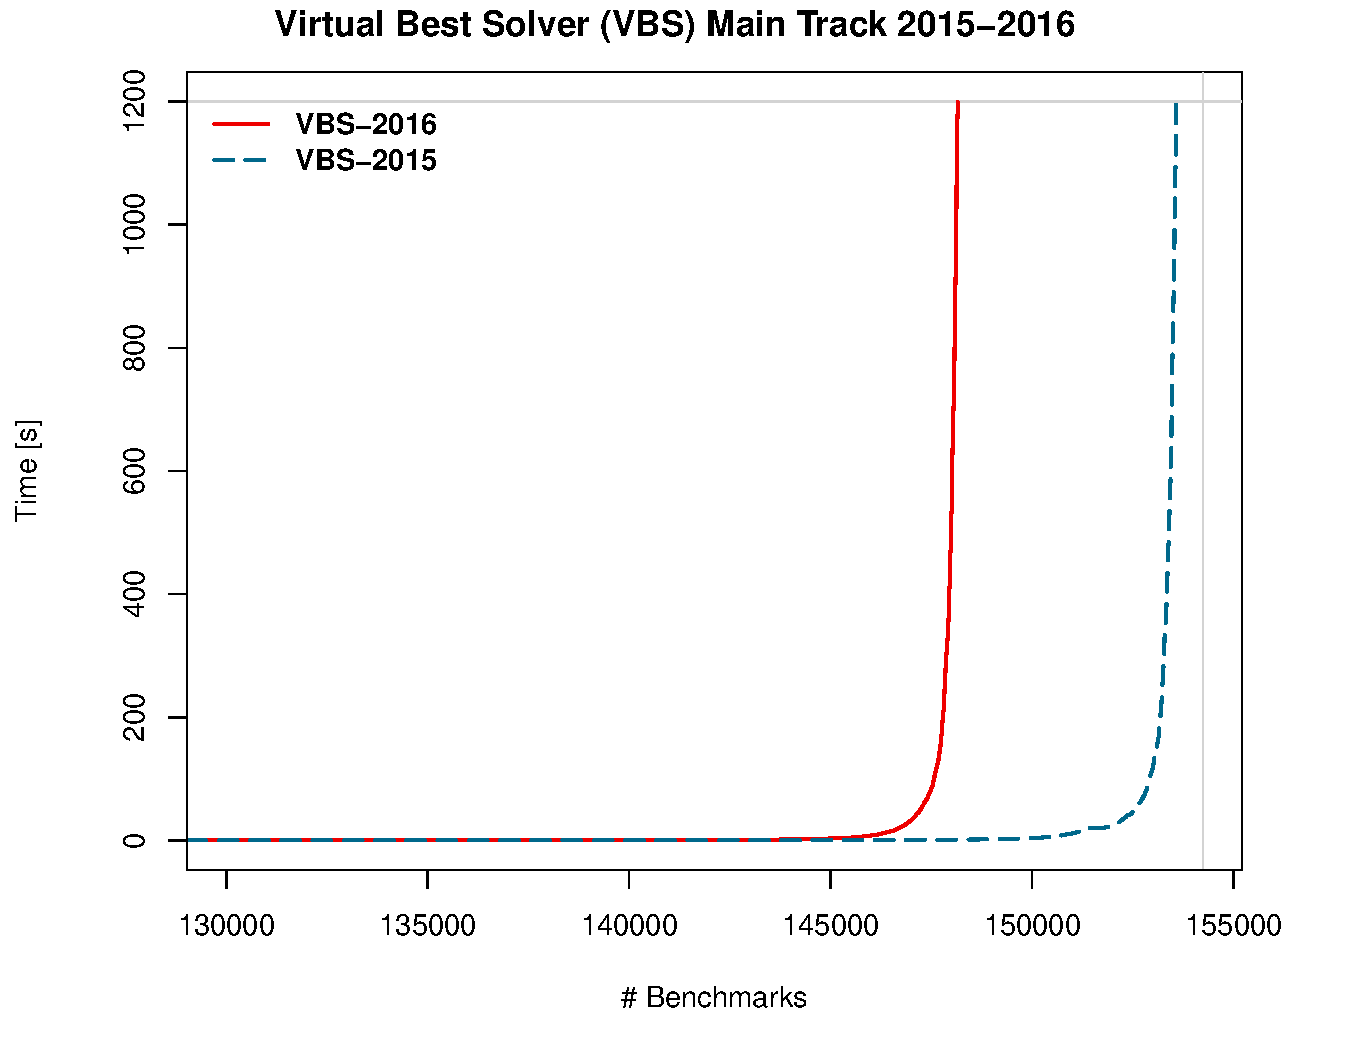
\includegraphics{%
      plot/pdf/cactus_plot-Virtual_Best_Solver_(VBS)_Main_Track_2015-2016.pdf}}
    \caption{2015 vs.~2016}
  \end{subfigure}
  \\[2ex]
  \begin{subfigure}[t]{0.5\textwidth}
    \scalebox{.35}{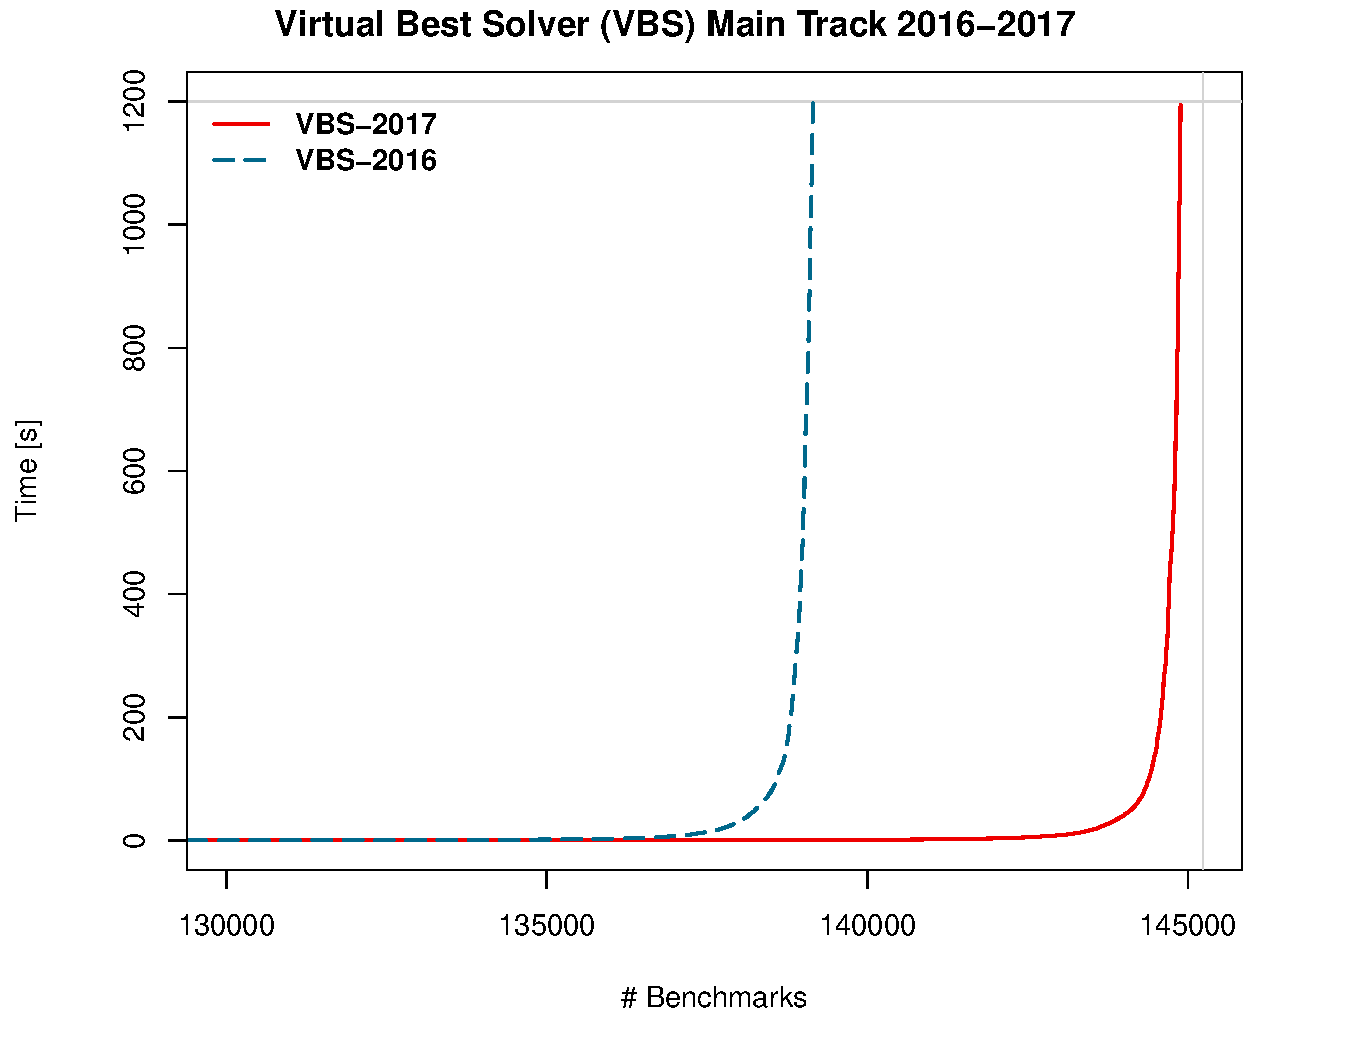
\includegraphics{%
      plot/pdf/cactus_plot-Virtual_Best_Solver_(VBS)_Main_Track_2016-2017.pdf}}
    \caption{2016 vs.~2017}
  \end{subfigure}
  \begin{subfigure}[t]{0.5\textwidth}
    \scalebox{.35}{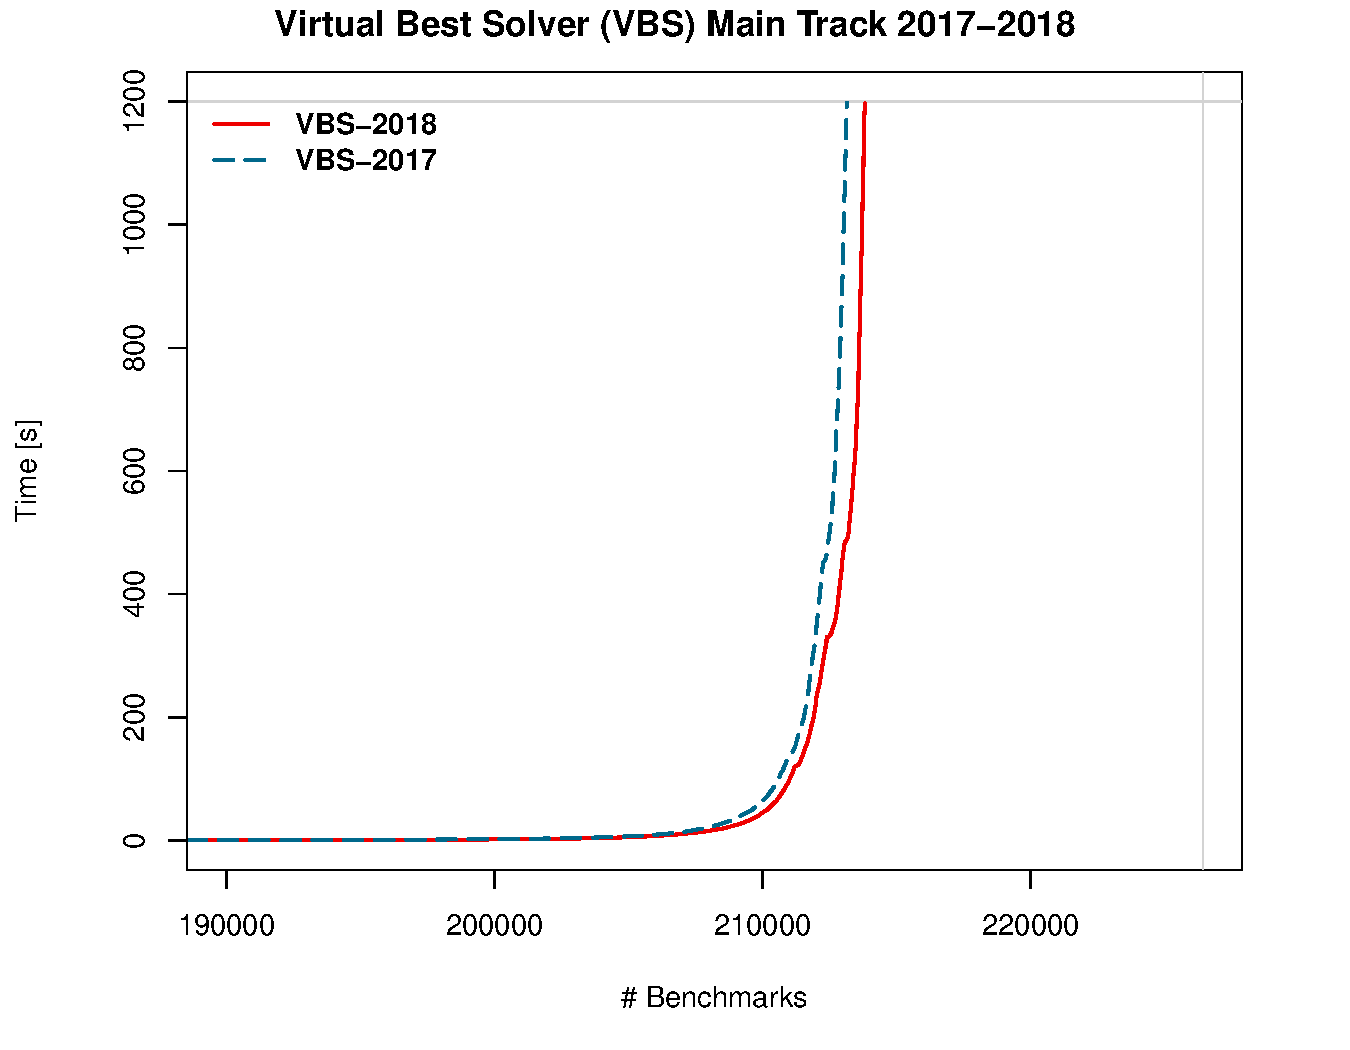
\includegraphics{%
    plot/pdf/cactus_plot-Virtual_Best_Solver_(VBS)_Main_Track_2017-2018.pdf}}
    \caption{2017 vs.~2018}
  \end{subfigure}
  \caption{VBS on common benchmarks for pairs of years of all logics in the
  \maintrack with a time limit of 1200s. Number of common benchmarks is
  indicated with a gray vertical line.}
  \label{fig:progress}
\end{figure}

\begin{figure}
  \centering
  \scalebox{.45}{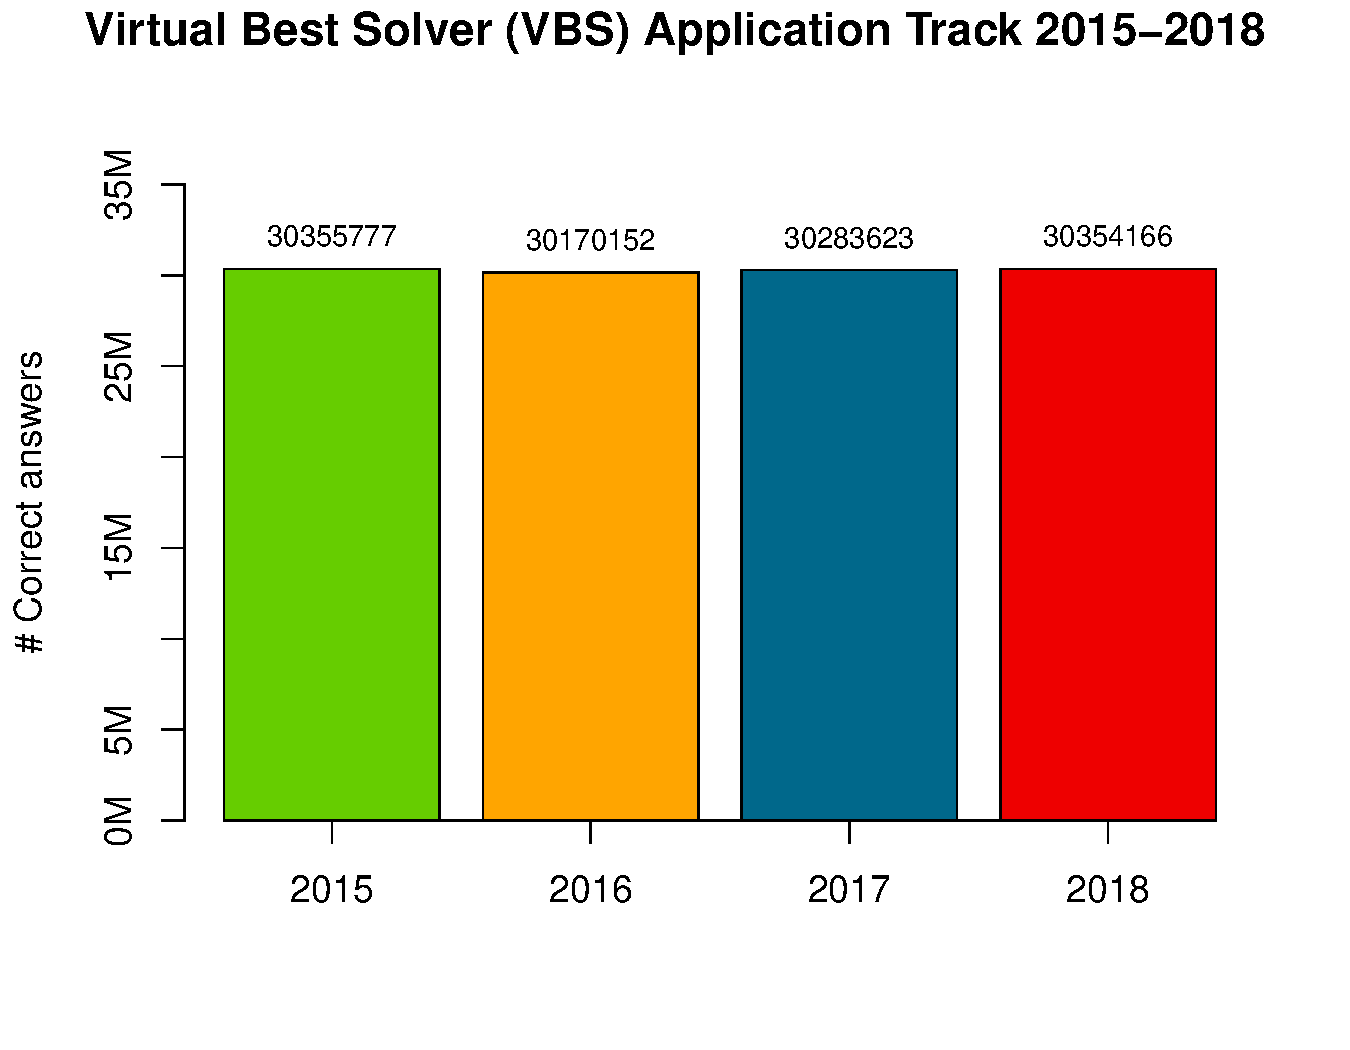
\includegraphics{%
  plot/pdf/bar_plot-Virtual_Best_Solver_(VBS)_Application_Track_2015-2018.pdf}}
  \vspace{-5ex}
  \caption{VBS in terms of correct \texttt{check-sat} answers
  (out of 30370517 total)
  within a time limit of 2400s
  on common benchmarks 2015-2018 of all logics in the \apptrack.}
  \label{fig:progress-all-app}
\end{figure}

\begin{figure}
  \centering
  \scalebox{.45}{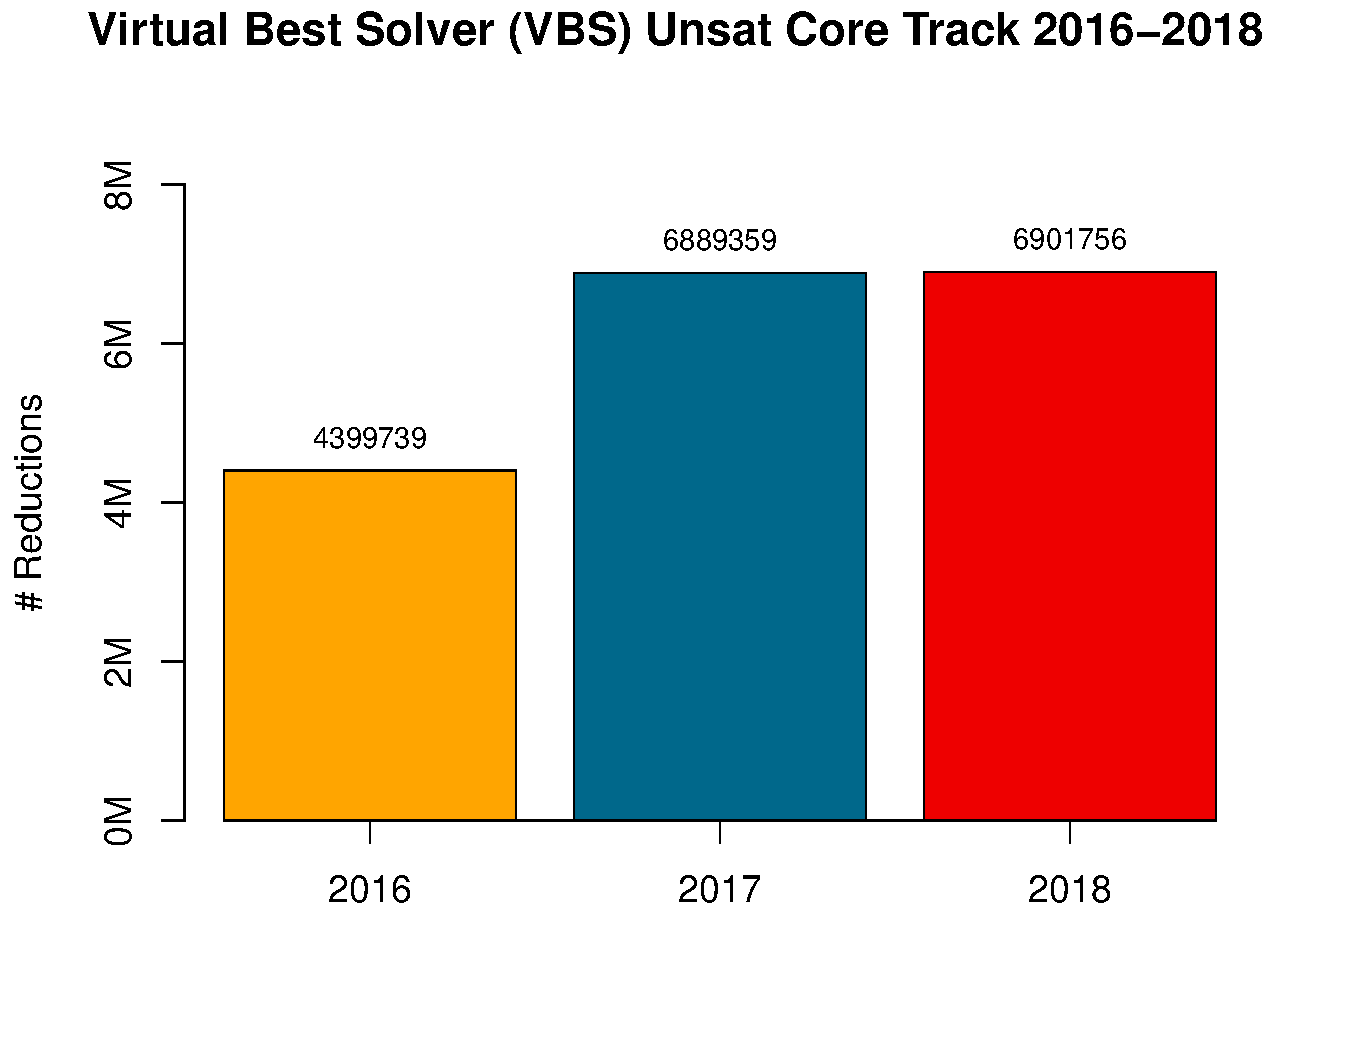
\includegraphics{%
  plot/pdf/bar_plot-Virtual_Best_Solver_(VBS)_Unsat_Core_Track_2016-2018.pdf}}
  \vspace{-5ex}
  \caption{VBS in terms of number of unsat core reductions
  within a time limit of 2400s
  on common benchmarks 2016-2018 of all logics in the \ucoretrack.}
  \label{fig:progress-all-uc}
\end{figure}

\section{Further Analysis}
\label{sec:analysis}

Beyond the competition rankings, the competition data provides ample
opportunity for further analysis.  Here, we report on three additional
aspects: progress in solver performance, number of uniquely solved
benchmarks, and use of parallelism in SMT solvers.

\subsection{Progress in Solver Performance}

The SMT Competition consists of several tracks with a multitude of divisions
per track.
Not all participating solvers enter all tracks, and the majority of
participants participates only in a handful of divisions.
To give a measure of overall progress in solver performance we
use the notion of \emph{virtual best solver} (VBS) over all divisions of all
three tracks.

For the \emph{\maintrack}, we determine the VBS as the best wall-clock
performance per (correctly solved) instance with the time limit of 1200s used
in the competitions 2017 and 2018. Figure~\ref{fig:progress-all} visualizes VBS
performance on common benchmarks from 2015-2018 as cactus plot.
Figure~\ref{fig:progress} shows VBS performance on common benchmarks over pairs
of consecutive years from 2014 to 2018.  Both plots show the wall-clock solving
time per instance over all instances, sorted by solving time.
%
Between 2014 (67426 benchmarks) and 2015 (154238 benchmarks),
the number of common benchmarks is 67070;
between 2015 and 2016 (154424 benchmarks) it is 154238;
between 2016 and 2017 (238758 benchmarks) it is 145236;
and between 2017 and 2018 (333241 benchmarks) it is 226429.
The number of solved instances on these sets of common benchmarks
increased from 2014 to 2015 by 0.1\%, from 2016 to 2017 by 3.9\%,
and from 2017 to 2018 by 0.3\%.
Interestingly, it decreased from 2015 to 2016 by 3.5\%.
This is mainly due to the fact that in 2015, more than 5600 benchmarks of
division QF\_FP where solved by one of the two participating configurations of
Z3 that no one else could solve, and in 2016 Z3 did not participate in this
division.

For the \emph{\apptrack}, we determine the VBS as the best performance
in terms of number of correct \texttt{check-sat} answers within the time limit
of 2400s (the time limit of the \apptrack in the competitions
2015-2018).
The total number of eligible \texttt{check-sat} queries (i.e., all queries with
status sat or unsat up to the first query with status unknown) on
common benchmarks from 2015-2018 is 30370517.
Figure~\ref{fig:progress-all-app} visualizes VBS performance on these
benchmarks as a bar plot.
In 2015, already 99.95\% of the eligible queries were answered correctly,
which naturally does not leave a lot of room for improvement.
In 2016, performance decreased by 185625 correct answers (0.61\%),
which can be entirely attributed to a performance degression
of Z3 on 2 benchmarks in the QF\_NIA division.
%(on which in 2016, CVC4 then
%performed best, and from 2017 onwards even as well as Z3 in 2015).

For the \emph{\ucoretrack}, we determine the VBS as the best performance in
terms of \emph{reduction}, i.e., the difference in the number of assertions
of the input formula and the unsat core, within the time limit
of 2400s (the time limit of the \ucoretrack in the competitions
2016-2018).
Figure~\ref{fig:progress-all-app} visualizes VBS performance on the common
benchmarks (91455 total) from 2016-2018 as a bar plot.
For 32377 of these benchmarks, extracting an unsat core is trivial since
they contain only one single \texttt{assert} command.
They are thus also not considered in the bar plot, since their maximum
possible reduction is trivially 0.


\subsection{Unique Solutions}

For each SMT solver, the number of uniquely solved benchmarks---that
is, the number of benchmarks that were solved by this solver only---is
a measure of how much the solver contributes to the state-of-the-art,
and the extent to which it is complementary to other solvers.  In
particular, if a solver that uniquely solves~$n$ benchmarks had not
participated in the competition, the virtual best solver would have
been able to solve~$n$ fewer benchmarks.
Table~\ref{table:unique-solutions} shows the number of uniquely solved
benchmarks for each \maintrack solver from 2015--2018.  (Multiple
versions of a solver are consolidated in this table, and answers that
were given by unsound solver versions are excluded.)

Solvers that rank highly in the competition-wide ranking
(Section~\ref{sec:floc}) often also solve many benchmarks uniquely,
but there are exceptions.  For instance, SMTInterpol has relatively
few unique solutions, despite achieving third place in the
competition-wide ranking in~2017 and~2018.  However, almost every
(sound) solver in the competition solves at least some benchmarks
uniquely, and hence contributes to the state-of-the-art.

The largest numbers in Table~\ref{table:unique-solutions} are due to
divisions in which there was only one sound solver: in~2016, MathSAT
was the only solver to support QF\_FP; in~2017, Z3 was the only sound
solver in QF\_FP; and in~2018, CVC4 was the only solver to support
QF\_SLIA, as well as the only sound solver in QF\_ABVFP.  Note that
divisions with fewer than two competing solvers do not affect the
competition-wide ranking.

\begin{table}
  \caption{Number of \maintrack benchmarks uniquely solved by each
    solver (by year)}
  \label{table:unique-solutions}
  \centering
  \begin{tabular}{lrrrr}
    \toprule
    Solver & 2015 & 2016 & 2017 & 2018 \\
    \midrule
    ABC               &       & 7     &       &        \\
    Alt-Ergo          &       &       &       & 1      \\
    AProVE            & 5     & 0     & 413   & 553    \\
    Boolector         & 37    & 25    & 97    & 62     \\
    COLIBRI           &       &       & 3     & 22     \\
    Ctrl-Ergo         &       &       &       & 12     \\
    CVC3              & 70    &       &       &        \\
    CVC4              & 4863  & 113   & 10258 & 100679 \\
    MapleSTP          &       & 0     &       &        \\
    {[}MathSAT{]}     & 21    & 28745 & 11    & 5      \\
    MinkeyRink        &       & 13    & 27    & 16     \\
    OpenSMT2          & 0     & 0     & 0     & 0      \\
    ProB              &       & 2     &       &        \\
    Q3B               &       & 0     & 89    & 0      \\
    raSAT             & 0     & 14    &       &        \\
    Redlog            &       &       & 4     &        \\
    SMT-RAT           & 12    & 0     & 85    & 2      \\
    SMTInterpol       & 1     & 1     & 5     & 4      \\
    SPASS-SATT        &       &       &       & 34     \\
    STP               & 4     & 1     & 4     & 5      \\
    toysmt            &       & 0     &       &        \\
    Vampire           &       & 130   & 753   & 652    \\
    veriT             & 7     & 19    & 55    & 57     \\
    XSat              &       &       & 0     &        \\
    Yices2            & 86    & 128   & 2379  & 1535   \\
    Z3                & 6118  & 244   & 40992 & 888    \\
    \midrule
    Total             & 11224 & 29442 & 55175 & 104527 \\
    \bottomrule
  \end{tabular}
\end{table}

\subsection{Use of Parallelism}

It is evident both from the division rankings
(Section~\ref{sec:division-rankings}) and the competition-wide ranking
(Section~\ref{sec:floc}) that there is very little difference between
sequential and parallel performance.  Even though parallel solvers may
use up to four times as much CPU time, sequential and parallel
division winners are most often identical, as are sequential and
parallel scores for the competition-wide ranking.

%TODO: discuss whether this can be attributed to the hardness
%distribution of benchmarks (cf. VBS plot)

In Table~\ref{table:parallelism}, we report the quotient of CPU time
over wall-clock time (summed up over all \maintrack benchmarks) for
each solver, as well as for all solvers combined.  When there were
multiple versions of a solver (such as a sequential and a parallel
version), only the highest value is shown.  We note that this quotient
is close to~1 for most solvers: only about 4--8 \maintrack solvers
each year were participating with a version that made use of
parallelism.

\begin{table}
  \caption{Quotient of CPU time over wall-clock time for each
    \maintrack solver (by year).  Values below~1.1 are shown in gray.}
  \label{table:parallelism}
  \centering
  \begin{tabular}{lrrrr}
    \toprule
    Solver & 2015 & 2016 & 2017 & 2018 \\
    \midrule
    ABC               &     & \textcolor{gray}{1.0} &     &     \\
    Alt-Ergo          &     &     &     & 3.0 \\
    AProVE            & \textcolor{gray}{1.0} & \textcolor{gray}{1.0} & \textcolor{gray}{0.8} & \textcolor{gray}{0.8} \\
    Boolector         & \textcolor{gray}{1.0} & \textcolor{gray}{1.0} & 1.1 & 1.3 \\
    COLIBRI           &     &     & \textcolor{gray}{1.0} & \textcolor{gray}{1.0} \\
    Ctrl-Ergo         &     &     &     & 4.0 \\
    CVC3              & \textcolor{gray}{1.0} &     &     &     \\
    CVC4              & 1.2 & 1.1 & 1.1 & \textcolor{gray}{1.0} \\
    MapleSTP          &     & 3.8 &     &     \\
    {[}MathSAT{]}     & \textcolor{gray}{1.0} & \textcolor{gray}{1.0} & \textcolor{gray}{1.0} & \textcolor{gray}{1.0} \\
    MinkeyRink        &     & 3.6 & 2.0 & 3.9 \\
    OpenSMT2          & 3.7 & \textcolor{gray}{1.0} & \textcolor{gray}{1.0} & \textcolor{gray}{1.0} \\
    ProB              &     & \textcolor{gray}{1.0} &     &     \\
    Q3B               &     & 2.9 & 2.9 & 3.0 \\
    raSAT             & \textcolor{gray}{1.0} & 2.0 &     &     \\
    Redlog            &     &     & \textcolor{gray}{1.0} &     \\
    SMT-RAT           & 1.3 & \textcolor{gray}{1.0} & \textcolor{gray}{1.0} & \textcolor{gray}{1.0} \\
    SMTInterpol       & 1.4 & 1.1 & 1.1 & 1.1 \\
    SPASS-SATT        &     &     &     & \textcolor{gray}{1.0} \\
    STP               & \textcolor{gray}{1.0} & 3.6 & 3.8 & 3.8 \\
    toysmt            &     & \textcolor{gray}{1.0} &     &     \\
    Vampire           &     & 3.4 & 3.9 & 4.0 \\
    veriT             & \textcolor{gray}{1.0} & \textcolor{gray}{1.0} & \textcolor{gray}{1.0} & \textcolor{gray}{1.0} \\
    XSat              &     &     & 1.8 &     \\
    Yices2            & \textcolor{gray}{1.0} & \textcolor{gray}{1.0} & \textcolor{gray}{1.0} & \textcolor{gray}{1.0} \\
    Z3                & \textcolor{gray}{1.0} & \textcolor{gray}{1.0} & \textcolor{gray}{1.0} & \textcolor{gray}{1.0} \\
    \midrule
    All solvers       & 1.0 & 1.3 & 1.3 & 1.3 \\
    \bottomrule
  \end{tabular}
\end{table}

\subsection{Focussing on Satisfiability or Unsatisfiability}

In many cases, an SMT application produces either mainly satisfiable or mainly
unsatisfiable queries to the SMT solver.  A typical example is model checking,
where a query is only satisfiable if a property of the model does not hold.  As
a consequence, some solvers may implement specialized techniques and
optimizations for the more frequent (the expected) case.
%
Therefore, it is interesting to ask whether the winners of divisions of a track
might have changed if benchmarks in that division had been restricted to one of
these results.  Tables~\ref{tab:results:sat}-\ref{tab:results:unsat} show the
changes in division winners if only satisfiable or unsatisfiable results are
given. This table is in reference to Table~\ref{tab:winners-main} and only
lists a solver if the result has changed. A non-competing solver is listed by
itself if it was not the overall best performing solver of that division but
now outperforms the winning competitive solver, and the winning competing
solver did not change.
It is interesting to note that we see some new solvers winning divisions that did not win any division in the main results. For example, Alt-Ergo solves the most satisfiable problems in AUFLIA and ALIA in 2018, and SMTInterpol performs very well on unsatisfiable problems in QF\_LIA.


We only consider the \maintrack here, which contains a mixture of problems that
are satisfiable and unsatisfiable.
\todo{give numbers in percent for years or refer to table where the numbers should be: {table:benchmarks-main-track}}
For the \apptrack, this analysis is less meaningful since a benchmarks usually
contains a multitude of both satisfiable and unsatisfiable incremental queries
(which may depend on each other).
For the \ucoretrack, only known unsatisfiable benchmarks from the \maintrack
are used, which renders this analysis useless for this track.



\begin{table}
  \caption{Alternative best solvers in the \maintrack if only \emph{satisfiable} benchmarks had been considered. These results are in reference to those given in Table~\ref{tab:winners-main}.}
  \label{tab:results:sat}
\centering
  \begin{tabular}{r@{\hskip 1em}>{\columncolor{white}[.25em][.5em]}c@{\hskip 1em}>{\columncolor{white}[.5em][.5em]}c@{\hskip 1em}>{\columncolor{white}[.5em][.5em]}c@{\hskip 1em}>{\columncolor{white}[.5em][0.5em]}c}
    \toprule
    Division         &  2015                &  2016                   &  2017                   &  2018                     \\
    \hline \hline
    ALIA             &                      &                         &                         & \cc{alt} Alt-Ergo         \\
    AUFLIA           & \cc{cvc3} CVC3       &                         &                         & \cc{alt} Alt-Ergo         \\
    AUFLIRA          &                      & \cc{cvc4} CVC4          & \cc{cvc4} CVC4          & \cc{alt} Alt-Ergo         \\
    AUFNIRA          & \nonc\nc{Z3}         & \cc{cvc4} CVC4 \nc{Z3}  & \cc{cvc4} CVC4 \nc{Z3}  & \nc{Z3}                   \\
    BV               &                      & \nc{Z3}                 & \cc{bool} Boolector     & \cc{bool} Boolector       \\
    LRA              &                      &                         & \cc{verit} veriT        &                           \\
    NIA              & \nonc \cc{cvc3} CVC3 &                         &                         &                           \\
    NRA              & \nonc \cc{cvc3} CVC3 & \cc{cvc4} CVC4          & \cc{cvc4} CVC4          & \cc{cvc4} CVC4 \nc{Z3}    \\
    QF\_ABV          &                      & \cc{yices} Yices2       & \cc{yices} Yices2       &                           \\
    QF\_AUFBV        & \cc{yices} Yices     & \cc{yices} Yices2       &                         & \cc{yices} Yices2         \\
    QF\_BV           &                      & \nc{Z3}/MinkeyRink      &                         &                           \\
    QF\_FP           &                      &                         &                         & \cc{cvc4} CVC4            \\
    QF\_LIA          & \nc{Z3}              &                         &                         &                           \\
    QF\_LRA          &                      &                         & \cc{yices} Yices2       & \cc{yices} Yices2         \\
    QF\_NIA          &                      & \cc{rat} SMT-RAT        &                         &                           \\
    QF\_NIRA         &                      &                         & \cc{cvc4} CVC4          &                           \\
    QF\_NRA          &                      &                         & \nc{Z3}                 &                           \\
    QF\_UFBV         &                      &                         &                         & \cc{yices} Yices2         \\
    QF\_UFIDL        & \nc{Z3}              & \nc{Z3}                 & \nc{Z3}                 & \cc{verit} veriT  \nc{Z3} \\
    QF\_UFNIA        & \nonc \cc{cvc3} CVC3 &                         & \cc{cvc4} CVC4          &                           \\
    UF               &                      & \cc{vamp} Vampire       &                         & \cc{vamp}Vampire/-        \\
    UFBV             &                      & \cc{bool} Boolector     &                         &                           \\
    UFDTLIA          &                      &                         & \nonc \cc{cvc4} CVC4    &                           \\
    UFLIA            & \nc{Z3}              &                         &                         &                           \\
    UFLRA            &                      & \cc{cvc4} CVC4          &                         &                           \\
    UFNIA            &                      & \cc{cvc4} CVC4          & \cc{cvc4} CVC4          & \cc{cvc4} CVC4            \\
    \bottomrule
  \end{tabular}
\end{table}

\begin{table}
  \caption{Alternative best solvers in the \maintrack if only \emph{unsatisfiable} benchmarks had been considered. These results are in reference to those given in Table~\ref{tab:winners-main}.}
  \label{tab:results:unsat}
  \centering
  \begin{tabular}{r@{\hskip 1em}>{\columncolor{white}[.25em][.5em]}c@{\hskip 1em}>{\columncolor{white}[.5em][.5em]}c@{\hskip 1em}>{\columncolor{white}[.5em][.5em]}c@{\hskip 1em}>{\columncolor{white}[.5em][0.5em]}c}
\toprule
Division        &  2015                  &  2016                     &  2017                 &  2018                   \\
\hline \hline
    BV          &                        & \cc{cvc4} CVC4            &                       &                         \\
    NIA         &                        & \cc{cvc4} CVC4            & \cc{vamp} Vampire     & \cc{vamp} Vampire       \\
    QF\_AUFBV   &                        &                           & \cc{cvc4} CVC4        &                         \\
    QF\_AUFNIA  & \nonc \nc{Z3}          & \nonc \nc{Z3}             &                       &                         \\
    QF\_BV      &                        &                           & -/Boolector           &                         \\
    QF\_IDL     & \cc{cvc4} CVC4         &                           & \nc{Z3}               & \cc{cvc4} CVC4 \nc{Z3}  \\
    QF\_LIA     & \cc{smti} SMTInterpol  & \cc{smti} SMTInterpol     & \cc{smti} SMTInterpol & \cc{smti} SMTInterpol   \\
    QF\_NIA     & \cc{cvc3} CVC3         &                           & \cc{yices} Yices2     &                         \\
    QF\_NRA     &                        &                           &                       & \cc{cvc4} CVC4          \\
    QF\_UFLIA   &                        &                           & \nc{Z3}               &                         \\
    QF\_UFNRA   &                        & \cc{cvc4} CVC4 \nc{Z3}    & \cc{cvc4} CVC4        & \cc{cvc4} CVC4 \nc{Z3}  \\
    UF          &                        &                           & \cc{cvc4} CVC4        & -/CVC4                  \\
    UFIDL       &                        & \cc{vamp} Vampire \nc{Z3} & \nc{Z3}               &                         \\
    UFLRA       &                        &                           & \cc{verit} veriT      & \cc{verit} veriT        \\
    \bottomrule
  \end{tabular}

\end{table}



%%%%%%%%%%%%%%%%%%%%
\subsection{Very Quick Solutions}

Different application domains of SMT typically impose a wide range of time
limits (from hours to seconds). In domains with very low time limits, these
limits are, in the incremental case, usually even defined per incremental
query.  With 20 and 40 minutes, the time limits used in the competition for all
tracks in all four years were relatively long and the same for all benchmarks,
thus agnostic to the application domain of a benchmark.  Hence, it is
interesting to investigate how the results change if we consider a much shorter
time limit.  Table~\ref{tab:results:24s} shows the results of virtually
imposing a time limit of 24 seconds\footnote{This time limit is used for the
new 24 seconds score introduced in SMT-COMP 2019 and was inspired by a use case
at Amazon.} in the \maintrack.  As in the previous, this highlights the
different winners under this new scheme only. Here we see STP winning a
division for the first time in our analysis (QF\_BV in 2016) and Yices2
performing well.

We only consider the \maintrack here, since for the other two tracks, the
results are less interesting.  In the \apptrack, for such low time limits we
are rather interested in a time limit per query, which we are unable to impose
on the existing data since it is not possible to extract wallclock run time
information per incremental query from the data of the competitions (as
mentioned above, StarExec does not record this information).  In the
\ucoretrack, the main focus is on producing small unsat-cores and solving times
are of secondary interest.  Additionally, benchmarks with known unsatisfiable
status from the \maintrack are used, and thus these results are already
available from the \maintrack analysis in Table~\ref{tab:results:24s}
(disregarding the fact that enabling unsat core production may slow down a
solver, depending on the technique).


\begin{table}
  \caption{Alternative best solvers in the \maintrack if the time limit had been 24 seconds.}
  \label{tab:results:24s}
  \centering

  \begin{tabular}{r@{\hskip 1em}>{\columncolor{white}[.25em][.5em]}c@{\hskip 1em}>{\columncolor{white}[.5em][.5em]}c@{\hskip 1em}>{\columncolor{white}[.5em][.5em]}c@{\hskip 1em}>{\columncolor{white}[.5em][0.5em]}c}
    \toprule
    Division   &  2015             &  2016                      &  2017                     &  2018                                  \\
    \hline \hline
    AUFLIA     &                   & \cc{vamp} Vampire \nc{Z3}  & \cc{verit} veriT          &                                        \\
    AUFLIRA    & \cc{cvc3} CVC3    &                            &                           & -/Alt-Ergo                             \\
    AUFNIRA    & \nonc \nc{Z3}     &                            &                           & \nc{Z3}                                \\
    BV         &                   &                            &                           & \cc{bool} Boolector/Boolector \nc{Z3}  \\
    NRA        &                   &                            &                           & \cc{cvc4} CVC4/CVC4 \nc{Z3}            \\
    QF\_ABV    &                   & \cc{yices} Yices2          &                           &                                        \\
    QF\_ANIA   &                   & \nonc \nc{Z3}              & \nonc \nc{Z3}             &                                        \\
    QF\_BV     & \cc{cvc4} CVC4    & \cc{stp} STP \nc{Z3}       &                           & -/Boolector                            \\
    QF\_LIA    & \cc{yices} Yices2 & \cc{yices} Yices2          & \cc{yices} Yices2         &                                        \\
    QF\_LRA    & \cc{yices} Yices2 & \cc{yices} Yices2          & \cc{yices} Yices2         & \cc{yices} Yices2                      \\
    QF\_NIA    &                   &                            & \cc{yices} Yices2         & \cc{yices} Yices2                      \\
    QF\_NIRA   &                   &                            & \cc{yices} Yices2 \nc{Z3} & \cc{yices} Yices2 \nc{Z3}              \\
    QF\_NRA    &                   &                            & \nc{Z3}                   &                                        \\
    QF\_UF     & \cc{verit} veriT  & \cc{verit} veriT           &                           &                                        \\
    QF\_UFNRA  &                   & \cc{cvc4} CVC4 \nc{Z3}     & \cc{cvc4} CVC4            & \nc{Z3}                                \\
    UF         &                   & \cc{vamp} Vampire          &                           &  \cc{vamp} Vampire/-                   \\
    UFBV       &                   & \cc{bool} Boolector        &                           &                                        \\
    UFIDL      &                   & \cc{vamp} Vampire \nc{Z3}  & \nc{Z3}                   &                                        \\
    UFLIA      &                   &                            &                           & \nc{Z3}                                \\
    UFLRA      &                   &                            & \cc{verit} veriT          & \cc{verit} veriT                       \\
    UFNIA      & \nonc \nc{Z3}     &                            &                           & \cc{cvc4} CVC4/\nc{Z3}                 \\
    \bottomrule
  \end{tabular}
\end{table}

\begin{table}
  \caption{Alternative best solvers in the \maintrack if the time limit had been 24 seconds. NEW}
  \label{tab:results:24s}
  \centering
  \scalebox{.82}{%
    \renewcommand{\arraystretch}{1.01}%
\begin{tabular}{r>{\columncolor{white}[.25em][.8em]}r@{\hskip .8em}|@{\hskip .5em}>{\columncolor{white}[.5em][.5em]}l>{\columncolor{white}[.5em][.8em]}r@{\hskip .8em}|@{\hskip .5em}>{\columncolor{white}[.5em][.5em]}l>{\columncolor{white}[.5em][.8em]}r@{\hskip .8em}|@{\hskip .5em}>{\columncolor{white}[.5em][0.5em]}l>{\columncolor{white}[.5em][.8em]}r@{\hskip .8em}|@{\hskip .5em}>{\columncolor{white}[.5em][0.5em]}l}
\toprule
Division &                 \multicolumn{2}{>{\columncolor{white}[.5em][.5em]}c}{2015} &                        \multicolumn{2}{>{\columncolor{white}[.5em][.5em]}c}{2016} &                        \multicolumn{2}{>{\columncolor{white}[.5em][.5em]}c}{2017} &                   \multicolumn{2}{>{\columncolor{white}[.5em][.5em]}c}{2018} \\
\midrule
AUFLIA   &                     \multicolumn{2}{>{\columncolor{white}[.5em][.5em]}c}{} &      \multicolumn{2}{>{\columncolor{white}[.5em][.5em]}c}{\cc{vamp} Vampire [Z3]} &            \multicolumn{2}{>{\columncolor{white}[.5em][.5em]}c}{\cc{verit} veriT} &                       \multicolumn{2}{>{\columncolor{white}[.5em][.5em]}c}{} \\
AUFLIRA  &  \multicolumn{2}{>{\columncolor{white}[.5em][.5em]}c}{\cc{cvc3} CVC3 [Z3]} &                            \multicolumn{2}{>{\columncolor{white}[.5em][.5em]}c}{} &                            \multicolumn{2}{>{\columncolor{white}[.5em][.5em]}c}{} &                                                     & \cc{alt} Alt-Ergo [Z3] \\
AUFNIRA  &  \multicolumn{2}{>{\columncolor{white}[.5em][.5em]}c}{\nonc \cc{cvc3} CVC3 [Z3]} &                            \multicolumn{2}{>{\columncolor{white}[.5em][.5em]}c}{} &                            \multicolumn{2}{>{\columncolor{white}[.5em][.5em]}c}{} &    \multicolumn{2}{>{\columncolor{white}[.5em][.5em]}c}{\cc{cvc4} CVC4 [Z3]} \\
BV       &                     \multicolumn{2}{>{\columncolor{white}[.5em][.5em]}c}{} &                            \multicolumn{2}{>{\columncolor{white}[.5em][.5em]}c}{} &                            \multicolumn{2}{>{\columncolor{white}[.5em][.5em]}c}{} &                               \cc{cvc4} CVC4 [Z3] & \cc{bool} Boolector [Z3] \\
NRA      &                     \multicolumn{2}{>{\columncolor{white}[.5em][.5em]}c}{} &                            \multicolumn{2}{>{\columncolor{white}[.5em][.5em]}c}{} &                            \multicolumn{2}{>{\columncolor{white}[.5em][.5em]}c}{} &    \multicolumn{2}{>{\columncolor{white}[.5em][.5em]}c}{\cc{cvc4} CVC4 [Z3]} \\
QF\_ABV   &                     \multicolumn{2}{>{\columncolor{white}[.5em][.5em]}c}{} &            \multicolumn{2}{>{\columncolor{white}[.5em][.5em]}c}{\cc{yices} Yices} &                            \multicolumn{2}{>{\columncolor{white}[.5em][.5em]}c}{} &                       \multicolumn{2}{>{\columncolor{white}[.5em][.5em]}c}{} \\
QF\_ANIA  &                     \multicolumn{2}{>{\columncolor{white}[.5em][.5em]}c}{} &         \multicolumn{2}{>{\columncolor{white}[.5em][.5em]}c}{\nonc \nonc \cc{cvc4} CVC4 [Z3]} &         \multicolumn{2}{>{\columncolor{white}[.5em][.5em]}c}{\nonc \cc{cvc4} CVC4 [Z3]} &                       \multicolumn{2}{>{\columncolor{white}[.5em][.5em]}c}{} \\
QF\_BV    &              \hspace*{3em}                                & \cc{cvc4} CVC4 &           \multicolumn{2}{>{\columncolor{white}[.5em][.5em]}c}{\cc{stp} STP [Z3]} &                            \multicolumn{2}{>{\columncolor{white}[.5em][.5em]}c}{} &                                                        & \cc{bool} Boolector \\
QF\_IDL   &     \multicolumn{2}{>{\columncolor{white}[.5em][.5em]}c}{\cc{yices} Yices} &            \multicolumn{2}{>{\columncolor{white}[.5em][.5em]}c}{\cc{yices} Yices} &                            \multicolumn{2}{>{\columncolor{white}[.5em][.5em]}c}{} &                       \multicolumn{2}{>{\columncolor{white}[.5em][.5em]}c}{} \\
QF\_LIA   &     \multicolumn{2}{>{\columncolor{white}[.5em][.5em]}c}{\cc{yices} Yices} &  \multicolumn{2}{>{\columncolor{white}[.5em][.5em]}c}{\cc{yices} Yices [MathSAT]} &  \multicolumn{2}{>{\columncolor{white}[.5em][.5em]}c}{\cc{yices} Yices [MathSAT]} &                       \multicolumn{2}{>{\columncolor{white}[.5em][.5em]}c}{} \\
QF\_LIRA  &                     \multicolumn{2}{>{\columncolor{white}[.5em][.5em]}c}{} &                            \multicolumn{2}{>{\columncolor{white}[.5em][.5em]}c}{} &            \multicolumn{2}{>{\columncolor{white}[.5em][.5em]}c}{\cc{yices} Yices} &       \multicolumn{2}{>{\columncolor{white}[.5em][.5em]}c}{\cc{yices} Yices} \\
QF\_LRA   &     \multicolumn{2}{>{\columncolor{white}[.5em][.5em]}c}{\cc{yices} Yices} &            \multicolumn{2}{>{\columncolor{white}[.5em][.5em]}c}{\cc{yices} Yices} &            \multicolumn{2}{>{\columncolor{white}[.5em][.5em]}c}{\cc{yices} Yices} &       \multicolumn{2}{>{\columncolor{white}[.5em][.5em]}c}{\cc{yices} Yices} \\
QF\_NIA   &                     \multicolumn{2}{>{\columncolor{white}[.5em][.5em]}c}{} &                            \multicolumn{2}{>{\columncolor{white}[.5em][.5em]}c}{} &            \multicolumn{2}{>{\columncolor{white}[.5em][.5em]}c}{\cc{yices} Yices} &       \multicolumn{2}{>{\columncolor{white}[.5em][.5em]}c}{\cc{yices} Yices} \\
QF\_NIRA  &                     \multicolumn{2}{>{\columncolor{white}[.5em][.5em]}c}{} &                            \multicolumn{2}{>{\columncolor{white}[.5em][.5em]}c}{} &       \multicolumn{2}{>{\columncolor{white}[.5em][.5em]}c}{\cc{yices} Yices [Z3]} &  \multicolumn{2}{>{\columncolor{white}[.5em][.5em]}c}{\cc{yices} Yices [Z3]} \\
QF\_NRA   &                     \multicolumn{2}{>{\columncolor{white}[.5em][.5em]}c}{} &                            \multicolumn{2}{>{\columncolor{white}[.5em][.5em]}c}{} &       \multicolumn{2}{>{\columncolor{white}[.5em][.5em]}c}{\cc{yices} Yices [Z3]} &                       \multicolumn{2}{>{\columncolor{white}[.5em][.5em]}c}{} \\
QF\_UF    &     \multicolumn{2}{>{\columncolor{white}[.5em][.5em]}c}{\cc{verit} veriT} &            \multicolumn{2}{>{\columncolor{white}[.5em][.5em]}c}{\cc{verit} veriT} &                            \multicolumn{2}{>{\columncolor{white}[.5em][.5em]}c}{} &                       \multicolumn{2}{>{\columncolor{white}[.5em][.5em]}c}{} \\
QF\_UFLIA &                                                         & \cc{yices} Yices &            \multicolumn{2}{>{\columncolor{white}[.5em][.5em]}c}{\cc{yices} Yices} &                            \multicolumn{2}{>{\columncolor{white}[.5em][.5em]}c}{} &                       \multicolumn{2}{>{\columncolor{white}[.5em][.5em]}c}{} \\
QF\_UFNRA &  \multicolumn{2}{>{\columncolor{white}[.5em][.5em]}c}{\nonc \cc{cvc4} CVC4 [Z3]} &         \multicolumn{2}{>{\columncolor{white}[.5em][.5em]}c}{\cc{cvc4} CVC4 [Z3]} &         \multicolumn{2}{>{\columncolor{white}[.5em][.5em]}c}{\cc{cvc4} CVC4 [Z3]} &  \multicolumn{2}{>{\columncolor{white}[.5em][.5em]}c}{\cc{yices} Yices [Z3]} \\
UF       &                     \multicolumn{2}{>{\columncolor{white}[.5em][.5em]}c}{} &           \multicolumn{2}{>{\columncolor{white}[.5em][.5em]}c}{\cc{vamp} Vampire} &                            \multicolumn{2}{>{\columncolor{white}[.5em][.5em]}c}{} &                                                         \cc{vamp} Vampire &  \\
UFBV     &                     \multicolumn{2}{>{\columncolor{white}[.5em][.5em]}c}{} &    \multicolumn{2}{>{\columncolor{white}[.5em][.5em]}c}{\cc{bool} Boolector [Z3]} &                            \multicolumn{2}{>{\columncolor{white}[.5em][.5em]}c}{} &                       \multicolumn{2}{>{\columncolor{white}[.5em][.5em]}c}{} \\
UFIDL    &                     \multicolumn{2}{>{\columncolor{white}[.5em][.5em]}c}{} &         \multicolumn{2}{>{\columncolor{white}[.5em][.5em]}c}{\cc{cvc4} CVC4 [Z3]} &         \multicolumn{2}{>{\columncolor{white}[.5em][.5em]}c}{\cc{cvc4} CVC4 [Z3]} &                       \multicolumn{2}{>{\columncolor{white}[.5em][.5em]}c}{} \\
UFLIA    &                     \multicolumn{2}{>{\columncolor{white}[.5em][.5em]}c}{} &                            \multicolumn{2}{>{\columncolor{white}[.5em][.5em]}c}{} &                            \multicolumn{2}{>{\columncolor{white}[.5em][.5em]}c}{} &    \multicolumn{2}{>{\columncolor{white}[.5em][.5em]}c}{\cc{cvc4} CVC4 [Z3]} \\
UFLRA    &                     \multicolumn{2}{>{\columncolor{white}[.5em][.5em]}c}{} &           \multicolumn{2}{>{\columncolor{white}[.5em][.5em]}c}{\cc{vamp} Vampire} &       \multicolumn{2}{>{\columncolor{white}[.5em][.5em]}c}{\cc{verit} veriT [Z3]} &       \multicolumn{2}{>{\columncolor{white}[.5em][.5em]}c}{\cc{verit} veriT} \\
UFNIA    &  \multicolumn{2}{>{\columncolor{white}[.5em][.5em]}c}{\nonc \cc{cvc4} CVC4 [Z3]} &                            \multicolumn{2}{>{\columncolor{white}[.5em][.5em]}c}{} &                            \multicolumn{2}{>{\columncolor{white}[.5em][.5em]}c}{} &                                 \cc{cvc4} CVC4 [Z3] & \cc{vamp} Vampire [Z3] \\
\bottomrule
\end{tabular}
  }
\end{table}


%%%%%%%%%%%%%%%%%
\subsection{Do Families Matter?}

In 2016 the \maintrack competition scoring was changed to weight the correctness score for benchmarks by the size of the family the benchmark belongs to. Here we ask what the winners would have been if this change had not been made. The answer to this question is given in Table~\ref{tab:results:total:solved}. Relatively few changes would have occurred. Unsurprisingly the differences are in the larger and more structured divisions.

Whilst producing these results we noticed that the description of what constitutes a family had been incorrectly interpreted by the scoring scripts in 2016-2018. After fixing this misinterpretation we note that only a single division winner changes - in 2017 AUFNIRA should have been won by 
\todo{who instead of who?}. As this is in the past we are choosing not to retroactively change the winner (and all tables in this paper reflect the previously published results) but the scripts have been fixed for future iterations of the competition.

\begin{table}
  \caption{Alternative best solvers in the \maintrack if families were not considered in computing scores (i.e., the 2015 scoring system were used)}
  \label{tab:results:total:solved}
  \centering
  \begin{tabular}{r@{\hskip 1em}>{\columncolor{white}[.25em][.5em]}c@{\hskip 1em}>{\columncolor{white}[.5em][.5em]}c@{\hskip 1em}>{\columncolor{white}[.5em][.5em]}c@{\hskip 1em}>{\columncolor{white}[.5em][0.5em]}c}
    \toprule
    Division & 2015 &  2016           &  2017                &  2018                  \\
    \hline\hline
    AUFNIRA  &      & \cc{cvc4} CVC4  &                      &                        \\
    UFIDL    &      & \nc{Z3}         &                      &                        \\
    BV       &      &                 & \cc{bool} Boolector  &                        \\
    QF\_LRA  &      &                 & \cc{yices} Yices2    & \cc{spass} SPASS-SATT  \\
    QF\_NIA  &      &                 & \cc{yices} Yices2    & \cc{yices} Yices2      \\
    QF\_BV   &      &                 &                      & -/Boolector            \\
    QF\_FP   &      &                 &                      & \cc{cvc4} CVC4         \\
  \bottomrule
  \end{tabular}
\end{table}


\begin{table}
  \caption{Alternative best solvers in the \maintrack if families were not considered in computing scores (i.e., the 2015 scoring system were used). NEW}
  \label{tab:results:total:solved}
  \centering
  {%
    \renewcommand{\arraystretch}{1.01}%

\begin{tabular}{r>{\columncolor{white}[.25em][.8em]}r@{\hskip .8em}|@{\hskip .5em}>{\columncolor{white}[.5em][.5em]}l>{\columncolor{white}[.5em][.8em]}r@{\hskip .8em}|@{\hskip .5em}>{\columncolor{white}[.5em][.5em]}l>{\columncolor{white}[.5em][.8em]}r@{\hskip .8em}|@{\hskip .5em}>{\columncolor{white}[.5em][0.5em]}l>{\columncolor{white}[.5em][.8em]}r@{\hskip .8em}|@{\hskip .5em}>{\columncolor{white}[.5em][0.5em]}l}
\toprule
Division & \multicolumn{2}{>{\columncolor{white}[.5em][.5em]}c}{2015}              &                 \multicolumn{2}{>{\columncolor{white}[.5em][.5em]}c}{2016} &                      \multicolumn{2}{>{\columncolor{white}[.5em][.5em]}c}{2017} &                   \multicolumn{2}{>{\columncolor{white}[.5em][.5em]}c}{2018} \\
\midrule
AUFNIRA  &     \multicolumn{2}{>{\columncolor{white}[.5em][.5em]}c}{\hspace*{5em}} &       \multicolumn{2}{>{\columncolor{white}[.5em][.5em]}c}{\cc{cvc4} CVC4} &                          \multicolumn{2}{>{\columncolor{white}[.5em][.5em]}c}{} &                       \multicolumn{2}{>{\columncolor{white}[.5em][.5em]}c}{} \\
BV       &     \multicolumn{2}{>{\columncolor{white}[.5em][.5em]}c}{}              &                     \multicolumn{2}{>{\columncolor{white}[.5em][.5em]}c}{} &  \multicolumn{2}{>{\columncolor{white}[.5em][.5em]}c}{\cc{bool} Boolector [Z3]} &                       \multicolumn{2}{>{\columncolor{white}[.5em][.5em]}c}{} \\
QF\_BV    &     \multicolumn{2}{>{\columncolor{white}[.5em][.5em]}c}{}             &                     \multicolumn{2}{>{\columncolor{white}[.5em][.5em]}c}{} &                                     \cc{mink} Minkeyrink &  \hspace*{3em}       &                           \hspace*{3em}                & \cc{bool} Boolector \\
QF\_FP    &     \multicolumn{2}{>{\columncolor{white}[.5em][.5em]}c}{}             &                     \multicolumn{2}{>{\columncolor{white}[.5em][.5em]}c}{} &                          \multicolumn{2}{>{\columncolor{white}[.5em][.5em]}c}{} &         \multicolumn{2}{>{\columncolor{white}[.5em][.5em]}c}{\cc{cvc4} CVC4} \\
QF\_IDL   &     \multicolumn{2}{>{\columncolor{white}[.5em][.5em]}c}{}             &                     \multicolumn{2}{>{\columncolor{white}[.5em][.5em]}c}{} &     \multicolumn{2}{>{\columncolor{white}[.5em][.5em]}c}{\cc{yices} Yices [Z3]} &                       \multicolumn{2}{>{\columncolor{white}[.5em][.5em]}c}{} \\
QF\_LRA   &     \multicolumn{2}{>{\columncolor{white}[.5em][.5em]}c}{}             &                     \multicolumn{2}{>{\columncolor{white}[.5em][.5em]}c}{} &                          \multicolumn{2}{>{\columncolor{white}[.5em][.5em]}c}{} &  \multicolumn{2}{>{\columncolor{white}[.5em][.5em]}c}{\cc{spass} SPASS-SATT} \\
QF\_NIA   &     \multicolumn{2}{>{\columncolor{white}[.5em][.5em]}c}{}             &                     \multicolumn{2}{>{\columncolor{white}[.5em][.5em]}c}{} &          \multicolumn{2}{>{\columncolor{white}[.5em][.5em]}c}{\cc{yices} Yices} &       \multicolumn{2}{>{\columncolor{white}[.5em][.5em]}c}{\cc{yices} Yices} \\
QF\_NRA   &     \multicolumn{2}{>{\columncolor{white}[.5em][.5em]}c}{}             &                     \multicolumn{2}{>{\columncolor{white}[.5em][.5em]}c}{} &                          \multicolumn{2}{>{\columncolor{white}[.5em][.5em]}c}{} &       \multicolumn{2}{>{\columncolor{white}[.5em][.5em]}c}{\cc{yices} Yices} \\
UFIDL    &     \multicolumn{2}{>{\columncolor{white}[.5em][.5em]}c}{}              &  \multicolumn{2}{>{\columncolor{white}[.5em][.5em]}c}{\cc{cvc4} CVC4 [Z3]} &                          \multicolumn{2}{>{\columncolor{white}[.5em][.5em]}c}{} &                       \multicolumn{2}{>{\columncolor{white}[.5em][.5em]}c}{} \\
\bottomrule
\end{tabular}
  }
\end{table}

%%%%%%%%%%%%%%%%%
\subsection{What Impact Did Adding Unknowns in the \maintrack Have?}

Until 2016, only benchmarks with known status were used in the \maintrack. In
2016, benchmarks with unknown status were evaluated separately, but not
considered in the overall results of the track.  Since 2017, non-incremental
benchmarks with unknown status were eligible for the \maintrack.
Table~\ref{tab:results:unknowns} shows alternative winners for 2017 and 2018 if
benchmarks with unknown status had not been included.



\begin{table}
  \caption{Alternative best solvers if benchmarks with unknown status had not bee included in 2017 onwards.}
  \label{tab:results:unknowns}
  \centering
    \begin{tabular}{r@{\hskip 1em}>{\columncolor{white}[.25em][.5em]}c@{\hskip 1em}>{\columncolor{white}[.5em][.5em]}c@{\hskip 1em}>{\columncolor{white}[.5em][.5em]}c@{\hskip 1em}>{\columncolor{white}[.5em][0.5em]}c}
    \toprule
    Division &  2017          &  2018                  \\
    \hline\hline
    AUFNIRA  & \cc{cvc4} CVC4 &                        \\
    QF\_NIRA & \nc{Z3}        & \cc{cvc4} CVC4 \nc{Z3} \\
    QF\_NRA  & \nc{Z3}        &                        \\
    UFDTLIA  & \cc{cvc4} CVC4 &                        \\
    BV       &                & \cc{bool} Boolector    \\
    QF\_FP   &                & \cc{cvc4} CVC4 \nc{Z3} \\
    UFNIA    &                & \cc{cvc4} CVC4         \\
    NRA      &                & -/\nc{Z3}              \\
    UF       &                & -/CVC4                 \\
  \bottomrule
  \end{tabular}
\end{table}


%%%%%%%%%%%%%%%%%%%%%%%%%%%%%%%%%%%%%%%%%%%%%%%%%%%%%%%%%%%%%%%%%%%%%%%%%%%%%%%%

\section{Conclusions}
\label{sec:conclusions}

The SMT Competition was instituted in~2005.  Thirteen years later, it
is a well-established event that garners wide interest from developers
and users of SMT solvers.  The competition continues to contribute to
its original goals, including adoption of the SMT-LIB format and
sparking further advances in SMT, and provides a yardstick of
performance for SMT solvers.

The last FLoC Olympiad was a period of significant growth for the SMT
Competition.  The average number of solver submissions increased
from~12 (for 2005--2014) to~26 (for 2015--2018).  The number of
SMT-LIB benchmarks used in the competition increased from~77,352
in~2014~\cite{CDW14} to 342,498 in 2018.  This is partly because new
benchmarks were added to the SMT Library, but also because benchmarks
with unknown status are now eligible for the competition, and because
the competition now uses all eligible benchmarks (rather than a
randomly selected subset).

Since the re-introduction of the \ucoretrack in~2016, the
competition again has three separate tracks.  This, together with new
logics in the SMT Library, has brought the total number of competition
divisions to 115 in~2018, up from just 40 divisions
in~2014~\cite{CDW14}.  The number of job pairs increased from 339,714
in~2014 to~1,776,062~in 2018, and the total wall-clock time in~2018
exceeded 7.6~years.  By these measures, the SMT Competition is one of
the largest competitions in automated reasoning.

The StarExec infrastructure has been vitally important in allowing the
competition to grow to its current size.  The competition organizers
have given the StarExec developers comprehensive feedback, and filed
dozens of feature requests and bug reports since 2013.  The
infrastructure has become increasingly stable; serious issues are now
rare.  When they did surface during ongoing competitions, they
received a swift response by the StarExec team (under the lead of
Aaron Stump).  This has been critical to the success of the
competition on more than one occasion.

Despite the substantial amount of computational resources available to
the competition through StarExec, the competition has reached a size
where future organizers will have to carefully consider the number of
participants and benchmarks each year, to determine time limits that
will allow the computational workload to complete before the SMT
Workshop.

Further development of the competition should be undertaken with care,
keeping in mind that major changes require not just the competition
organizers, but also participants to adapt.  Immediate action items
for next year's organizers are
\begin{itemize}
\item the inclusion of {\tt check-sat} commands with unknown status in
  the \apptrack, and
\item the definition of competition-wide rankings for the \apptrack 
  and \ucoretrack.
\end{itemize}

For the inclusion of new tracks or divisions, a two-phase approach has
proven successful.  A new division is first declared
\emph{experimental}, meaning that results will be reported but no
official winner will be announced.  This allows competition organizers
and participants to gain valuable experience, while reducing the
impact of mistakes.  If successful, the division may then become
regular in the following year.

Organizing the competition is a non-trivial amount of work.  For
instance, the competition tools (such as the benchmark scrambler and
trace executor) often require updating when new divisions are added,
or when changes are made to StarExec.  One could imagine adding
further tracks to the competition (e.g., for proof-producing solvers,
or for variants such as max-SMT), but the effort required to support
such tracks will need to be balanced against their added value.

To ensure that the competition results are practically relevant, it is
important that the SMT Library contains benchmarks that cover a wide
range of applications.  To this end, we again encourage users of SMT
solvers to submit new and interesting benchmarks to the library,
especially for underrepresented logics.  This is not just a valuable
contribution to the community, but also---since these benchmarks will
then be used in the competition---a straightforward way to incentivize
solver developers to tune their solvers accordingly.

\paragraph{Acknowledgments}

We would like to thank Aaron Stump for allowing the SMT Competition to
run on StarExec; the SMT-LIB maintainers, namely Clark Barrett, Pascal
Fontaine, Aina Niemetz and Mathias Preiner, for preparing the annual
SMT-LIB release; all contributors of new benchmarks to the SMT
Library; and, last but not least, all solver developers who entered
their solver into the competition.

%%%%%%%%%%%%%%%%%%%%%%%%%%%%%%%%%%%%%%%%%%%%%%%%%%%%%%%%%%%%%%%%%%%%%%%%%%%%%%%%

\bibliographystyle{plainbv}
\bibliography{SMT-COMP}

\end{document}

%%%%%%%%%%%%%%%%%%%%%%%%%%%%%%%%%%%%%%%%%%%%%%%%%%%%%%%%%%%%%%%%%%%%%%%%%%%%%%%%

% Local Variables:
% ispell-local-dictionary: "american"
% mode: LaTeX
% mode: flyspell
% LocalWords: concours hors logics satisfiability SMT Tjark
% End:
